\pdfoutput=1  % tells arXiv to compile with pdfLaTeX
\documentclass[11pt]{article}

% ---------- packages ----------
\usepackage[a4paper,margin=1in]{geometry}
\usepackage{amsmath,amssymb,amsthm}
\usepackage{graphicx}
\usepackage{booktabs}
\usepackage{xcolor}
\usepackage[numbers,sort&compress]{natbib}
\usepackage[colorlinks=true,linkcolor=blue,citecolor=blue,urlcolor=blue]{hyperref}
\usepackage{tabularx}
\usepackage{tikz}
\usetikzlibrary{arrows.meta}

% ---------- small helpers ----------
\newcommand{\code}[1]{\colorbox{gray!12}{\texttt{\vphantom{Ag}#1}}}
\newcommand{\todo}[1]{\textcolor{red}{[#1]}}

% ---------- theorem environments ----------
\newtheorem{theorem}{Theorem}[section]
\newtheorem{lemma}[theorem]{Lemma}
\newtheorem{proposition}[theorem]{Proposition}
\newtheorem{definition}[theorem]{Definition}

\begin{document}
\thispagestyle{plain}

\noindent
\includegraphics[height=1.3cm]{figures/university_logo.png}%
\par\vspace{4pt}
\noindent\rule{\textwidth}{0.4pt}

\vspace{3.5em}

\renewcommand{\thefootnote}{\fnsymbol{footnote}}
\begin{center}
  {\LARGE Isabelle Pool Server: a pooled verification service\\for prover training and multi-agent proving\par}
  \vspace{1.6em}
  {\large
    Xuanwei Ren\footnotemark[1]\quad
    Wenda Li\footnotemark[2]\par}
  \vspace{1.6em}
\end{center}
\footnotetext[1]{School of Informatics, University of Edinburgh, UK.
  Email: \texttt{s2415809@ed.ac.uk}}
\footnotetext[2]{School of Informatics, University of Edinburgh, UK.
  Email: \texttt{wenda.li@ed.ac.uk}}
\renewcommand{\thefootnote}{\arabic{footnote}}
\setcounter{footnote}{0}

\vspace{1em}

% ======================================================================
\begin{abstract}
We present Isabelle Pool Server (IPS), a verification service for
Isabelle/HOL built for two users that existing Isabelle connectors do not
serve: training loops for LLM provers and groups of agents sharing one
prover host. IPS keeps a pool of warm Isabelle sessions, each a headless
instance of PIDE, Isabelle's document model, and leases them to clients
over HTTP, one client per session at a time. Every call runs under a
wall-clock budget. A session offers three verification modes, one command
at a time, a proof chunk checked as one transaction, and a whole-file
build as the final arbiter, together with checkpoints and rollback.
Clients use a Python client or one of two bundled MCP servers. We
measured IPS and PIDE MCP, the other headless PIDE connector, on one
128\,GB host with 1 to 32 concurrent sessions on three heaps. A session
costs 0.9--1.3\,GB under IPS and 1.3--1.5\,GB under PIDE MCP in its
intended one-process shape, or 2.7--3.7\,GB when each agent runs its own
PIDE MCP process. Under a 48\,GB limit, IPS admits 27 HOL-Analysis
sessions and refuses the next with a reason; one PIDE MCP process per
agent reaches 13, and the kernel then kills four of them. A released IPS
session is handed to the next client in 2\,ms. On the 93 theories of
HOL-Analysis, restoring a checkpoint takes 4\,ms where replaying to the
same proof state takes 8 to 93\,s, the in-session verdict agreed with a
cold build on all 890 checks, 597 of them on broken proofs, every looping
step returned at its budget, and 32 workers verified 3\,181 chunks per
minute. IPS is free software:
\url{https://github.com/FullBackward/Isabelle-Pool-Server}.
\end{abstract}

% ======================================================================
\section{Introduction}

Machines now drive proof assistants more than people do, in two ways.
Training an LLM prover means verifying thousands of candidate proof steps
per hour. Every Isabelle prover since LISA has done this through
PISA-style read-eval-print loops, one Isabelle process per
worker~\cite{jiang2021lisa,jiang2022thor,jiang2023dsp,mikula2024magnushammer},
and their authors name the cost of attempts as the limiting
factor~\cite{jiang2023dsp,mikula2024magnushammer}. Running coding agents
means many agents reaching the prover over the Model Context Protocol
(MCP)~\cite{anthropic2024mcp} and sharing machines that can each hold a
few Isabelle heaps. Lean has infrastructure for both: Kimina Lean Server
pools REPL workers for reinforcement
learning~\cite{santos2025kimina,deepseek2024proverv15}, and AXLE hosts
isolated, strictly checked verification for agents and training
alike~\cite{xin2026axle}. Isabelle has neither. Its connectors expose
PIDE, the document model behind Isabelle's editors~\cite{wenzel2014pide},
to one agent at a time: Isabelle/Q~\cite{awslabs2026autocorrode} inside a
human's editor session, PIDE MCP~\cite{kappelmann2026pidemcp} as a
headless process per agent.

The two workloads need the same service. A training loop branches at a
proof state, discards most of what it tries, and must bound every step so
that no attempt stalls a worker. It needs a verdict it can trust, because
a verifier that accepts an unfinished proof corrupts the
reward~\cite{deepseek2025proverv2,xin2026axle}. An agent harness needs
each agent isolated from the others, a session ready on request, calls
that return within a known time, and access over the network. Both need
a component that decides who gets a session, when it is taken back, and
what happens when memory runs out.

IPS is a pooled verification service that makes those decisions. It keeps
a pool of warm headless PIDE sessions, leases them to clients over HTTP,
reclaims idle and abandoned leases, and gates admission on memory. Because
a PIDE session is a document rather than a command
stream~\cite{wenzel2012repl}, IPS offers what a REPL pool cannot: a failed
attempt is rolled back as if never submitted, a checkpoint is restored
exactly, a proof chunk is checked as one edit with parallel proof checking
on, and a whole file can be rebuilt from a cold heap as the final verdict.
Every wait on the prover runs under a wall-clock budget. Training
harnesses use a Python client; agents use one of two bundled MCP servers,
one that verifies submitted proof chunks and one that follows a theory
file the agent edits on disk.

We write for two readers, the \emph{training reader} who builds or
evaluates an LLM prover and the \emph{operator} who runs a shared Isabelle
host, and we state each reader's requirements as metrics before reporting
on them (Section~\ref{sec:readers}). Our contributions are:
\begin{enumerate}
  \item \textbf{A pooled PIDE service.} Leased sessions with budgets,
    transactional chunk verification, checkpoints and rollback, a cold
    build as arbiter, memory-gated admission, and a Python client plus two
    MCP servers (Section~\ref{sec:arch}).
  \item \textbf{Measurements for both readers.} Throughput, latency,
    branch cost, verdict agreement and bounded steps on the HOL-Analysis
    library for the training reader; memory per session, acquire latency,
    behaviour under a memory limit and crash containment for the operator;
    all on one 128\,GB host, with PIDE MCP measured under the same
    conditions (Sections~\ref{sec:training}, \ref{sec:serving}
    and~\ref{sec:comparison}).
  \item \textbf{A comparison with PIDE MCP.} The design choices that
    separate the two headless PIDE connectors, what each can do that the
    other cannot, and a feature inventory (Section~\ref{sec:comparison},
    Appendix~\ref{app:inventory}).
  \item \textbf{An open implementation.} The service, the experiment
    harness and the raw results are public (Appendix~\ref{app:bench}).
\end{enumerate}
Section~\ref{sec:position} places IPS among
Isabelle connectors; Section~\ref{sec:limitations} lists its limits.

% ======================================================================
\section{Requirements and metrics}
\label{sec:readers}

\subsection{Two readers}

The \textbf{training reader} builds or evaluates an LLM prover. Their
loop samples candidate steps, submits them, and learns from the verdicts.
They judge IPS by what it does to that loop: verified steps per hour,
time per verdict, the cost of branching, and whether ``proved'' can be
trusted as a reward.

The \textbf{operator} runs one Isabelle host that several agents or
harnesses share. They judge IPS by capacity and by conduct under load:
sessions per host, wait for a session, heap rebuilds, and behaviour when
memory runs out.

A third reader, the single agent working interactively beside a human, is
the one the PIDE MCP preprint's desiderata
describe~\cite{kappelmann2026pidemcp}. IPS does not primarily serve that
reader; Sections~\ref{sec:comparison} and~\ref{sec:position} make the
comparison.

\subsection{Metrics}

Table~\ref{tab:metrics} turns each reader's questions into the metrics
that Sections~\ref{sec:training} and~\ref{sec:serving} report, with the
procedure for each in Appendix~\ref{app:bench}. This version measures
every metric except the cache hit rate. Agent success on
a benchmark measures the agent and its prompt rather than the service, so
it appears only as a worked example in Section~\ref{sec:position}.

\begin{table}[t]
\centering\small
\begin{tabularx}{\textwidth}{@{}>{\raggedright\arraybackslash}X l >{\raggedright\arraybackslash}X l@{}}
\toprule
Question & Metric & Measured as & Status \\
\midrule
\multicolumn{4}{@{}l}{\emph{Training reader} (Section~\ref{sec:training})} \\
How many verified rollouts per hour? & throughput & \code{verify\_chunk} calls per minute and scripted rollouts per hour, against worker count & measured \\
How long does one verify call take? & latency & p50 and p95 of \code{verify\_chunk}, by chunk size & measured \\
Can I branch and backtrack cheaply? & branch cost & restore time against replaying to the same proof state & measured \\
Does ``proved'' in-session mean proved cold? & agreement & in-session verdict against a cold build, on the corpus and on broken proofs & measured \\
Can one bad step stall a worker? & bounded step & looping steps returned at their budget; recovery; effect on other workers & measured \\
\midrule
\multicolumn{4}{@{}l}{\emph{Operator} (Section~\ref{sec:serving})} \\
How many sessions fit in a host? & capacity & memory per session at steady state, by heap; sessions per 100\,GB & measured \\
How long until a client gets a session? & acquire latency & warm hit, cold start and heap build, separately & measured \\
How often is a heap rebuilt? & cache hit rate & heap cache hits and misses over a project mix & not measured \\
What happens when memory runs out? & pressure & admission refusals, evictions, kernel kills, recovery time & measured \\
Are agents isolated from each other? & isolation & crash containment: do the other sessions answer? & measured \\
\bottomrule
\end{tabularx}
\caption{Each reader's questions, the metric that answers each, how it is measured, and whether this version reports it.}
\label{tab:metrics}
\end{table}

% ======================================================================
\section{Service overview}
\label{sec:arch}

This section describes IPS as a client sees it. Figure~\ref{fig:arch}
shows the parts.

\begin{figure}[!htb]
\centering
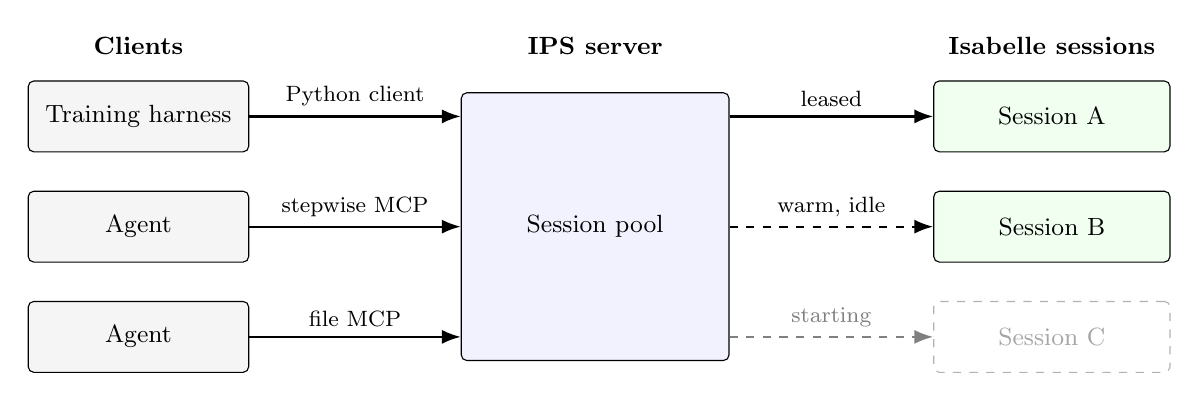
\begin{tikzpicture}[
  x=1cm, y=1cm, font=\small,
  box/.style={draw, rounded corners=2pt, align=center, minimum height=9mm, inner sep=4pt},
  client/.style={box, fill=gray!8,  minimum width=28mm},
  pool/.style={box, fill=blue!5,   minimum width=34mm, minimum height=34mm},
  session/.style={box, fill=green!6, minimum width=30mm},
  faded/.style={box, fill=white, draw=gray!60, text=gray!70, dashed, minimum width=30mm},
  arr/.style={-{Latex[length=2.4mm]}, thick},
  lbl/.style={font=\footnotesize},
  column/.style={font=\small\bfseries}
]
% clients
\node[client] (c1) at (0, 0)   {Training harness};
\node[client] (c2) at (0,-1.4) {Agent};
\node[client] (c3) at (0,-2.8) {Agent};
\node[column] at (0, 0.9) {Clients};
% pool
\node[pool] (pool) at (5.8,-1.4) {Session pool};
\node[column] at (5.8, 0.9) {IPS server};
% sessions
\node[session] (s1) at (11.6, 0)   {Session A};
\node[session] (s2) at (11.6,-1.4) {Session B};
\node[faded]   (s3) at (11.6,-2.8) {Session C};
\node[column] at (11.6, 0.9) {Isabelle sessions};
% clients -> pool
\draw[arr] (c1.east) -- (pool.west |- c1.east) node[midway, above, lbl] {Python client};
\draw[arr] (c2.east) -- (pool.west |- c2.east) node[midway, above, lbl] {stepwise MCP};
\draw[arr] (c3.east) -- (pool.west |- c3.east) node[midway, above, lbl] {file MCP};
% pool -> sessions
\draw[arr]               (pool.east |- s1.west) -- (s1.west) node[midway, above, lbl] {leased};
\draw[arr, dashed]       (pool.east |- s2.west) -- (s2.west) node[midway, above, lbl] {warm, idle};
\draw[arr, dashed, gray] (pool.east |- s3.west) -- (s3.west) node[midway, above, lbl, text=gray] {starting};
\end{tikzpicture}
\caption{A client's view of IPS. A training harness talks to the pool
  through the Python client; an agent through one of the two bundled MCP
  servers. The pool holds warm Isabelle sessions and leases each to one
  client at a time (session A). A released session stays warm for the
  next client with the same imports (session B). A new session starts
  only when no warm one matches and the host has memory for it
  (session C). Every call into a session runs under a time budget.}
\label{fig:arch}
\end{figure}

\subsection{Sessions and leases}

A client works with a \emph{session}: a running Isabelle, loaded with the
imports the client asked for, holding one theory the client builds up by
submitting text. The client never starts Isabelle and never sees a file.
Three properties of a session are fixed: its imports cannot change, its
document is one theory rather than a project, and it belongs to one
client for the life of its lease. A training harness reaches sessions
through the Python client; an agent through the \emph{stepwise} MCP
server, which verifies chunks the agent submits, or the \emph{file} MCP
server, which follows a theory file the agent edits with its own tools.

\subsection{Acquiring a session}

The client names the imports it needs. If an idle session with those
imports exists, it is leased at once; a warm hit takes 2\,ms
(Section~\ref{sec:serving-measured}). Otherwise the pool starts one, which
takes 2 to 6 seconds on a built heap, or refuses with an explanation if
the host is short of memory. Imports from the Isabelle distribution are
always available. Imports from the client's own project need a heap that
IPS builds once on request and reuses until the project's sources change.
Leases expire and idle sessions are reclaimed, so a client that fails to
release does not hold a session indefinitely.

\subsection{Verification modes}

\begin{itemize}
  \item \emph{One command at a time}, for a loop that wants the proof
    state after each step. A failed or timed-out step is undone.
  \item \emph{A proof chunk} (\code{verify\_chunk}): a block of Isar
    submitted at once. IPS checks it as one unit, reports each command's
    status, and states whether the proof is still open and whether
    \code{sorry} was used. If any command fails, the whole block is
    undone. This is the call a training loop uses.
  \item \emph{A whole file}, rebuilt from scratch in a fresh Isabelle,
    for a verdict that must be final. It is slower, stateless and cached.
\end{itemize}
Between submissions the client can read goals, open proofs, facts in
scope, or a Sledgehammer suggestion without changing the document; take a
\emph{checkpoint} and later \emph{restore} it, so a search branches and
backtracks without a new session; or \emph{roll back} the last submission.

\subsection{Verdict semantics}

IPS separates ``did anything error'' from ``is the theorem proved''. A
chunk \emph{succeeds} when no command in it errored. It is \emph{proved}
when it succeeded, left no proof open, and used no \code{sorry}; the
client reads this from three flags in the response. When a verdict
matters beyond the current loop, the whole-file check is the arbiter,
because an in-session check can accept a step that a fresh build rejects.

\subsection{Time budgets}

Every call that waits on Isabelle carries a budget, chosen by the client
and enforced by the server. A call that exceeds its budget returns a
timeout, undoes what it submitted, and leaves the session usable. No
submission can hold a session or a worker indefinitely. This guarantee is
what a training loop and an agent harness both rely on, and it is the
main point on which IPS differs from an interactive connector such as
PIDE MCP, which bounds nothing by design (Section~\ref{sec:comparison}).
Appendix~\ref{app:code} explains how the server keeps these guarantees;
Appendix~\ref{app:deploy} how it is configured.

% ======================================================================
\section{Training workloads}
\label{sec:training}

This section is for the training reader. It states what a training loop
needs from a verification service, how IPS provides it, and what we
measured.

\subsection{Requirements}

A training loop, whether reinforcement learning, expert iteration or
search, has one shape: sample candidate steps, submit them, learn from
the verdicts, repeat. It needs four things from the service.

\paragraph{Verdicts at the sampler's rate.} Thor issues up to 300 model
queries per theorem~\cite{jiang2022thor}; DeepSeek-Prover-V2 samples 32
candidate proofs per problem at every reinforcement-learning
step~\cite{deepseek2025proverv2}. A Lean pool answers one such request in
about 0.05 seconds on 64 cores~\cite{santos2025kimina}; that is the
reference point for an Isabelle service.

\paragraph{Cheap branching at a proof state.} Best-first and tree search
in Thor~\cite{jiang2022thor}, Magnushammer~\cite{mikula2024magnushammer}
and DeepSeek-Prover-V1.5~\cite{deepseek2024proverv15} all branch. In a
REPL, every branch is a replay from the start or a fresh process.

\paragraph{A bound on every step.} Every system in this lineage bounds
each prover call, from 2 seconds in
Magnushammer~\cite{mikula2024magnushammer} to 300 in
DeepSeek-Prover~\cite{deepseek2024proverv15}, because one looping tactic
otherwise removes a worker from the pool.

\paragraph{A verdict that means what the reward assumes.}
DeepSeek-Prover-V2 traced inflated benchmark results to a Lean bug that
failed to report \code{sorry}~\cite{deepseek2025proverv2}; AXLE's strict
verifier exists because compilation alone accepts \code{sorry}, unsound
axioms and restated theorems~\cite{xin2026axle}. IPS had its own
instance: an in-session check once accepted a \code{metis} call that a
fresh build rejected.

\subsection{Design}

The loop acquires a session per worker with the imports of its problems
and keeps it while the imports stay the same. Each
candidate is submitted as a chunk. The per-command report names the step
that failed, and a failed chunk leaves the session unchanged, so the next
candidate goes to the same state without cleanup. To branch, the loop
takes a checkpoint at the proof state, tries a continuation, and restores
the checkpoint before the next; both are document edits, not session
restarts. Every submission carries a budget; one that exceeds it is
undone and reported as a timeout, so no worker is lost to a runaway step.
The reward reads three flags from the chunk report: success, no open
proof, no \code{sorry}. For evaluation, where a verdict is final, the
loop submits the completed theory to the whole-file check, which rebuilds
it from a cold heap. For batch evaluation without session state, the
stepwise MCP server's \code{verify\_batch} tool and the HTTP batch route
fan a set of candidates out across the pool and return their verdicts
together. Figure~\ref{fig:rollout} shows the loop as a client sees it.

\begin{figure}[!htb]
\centering
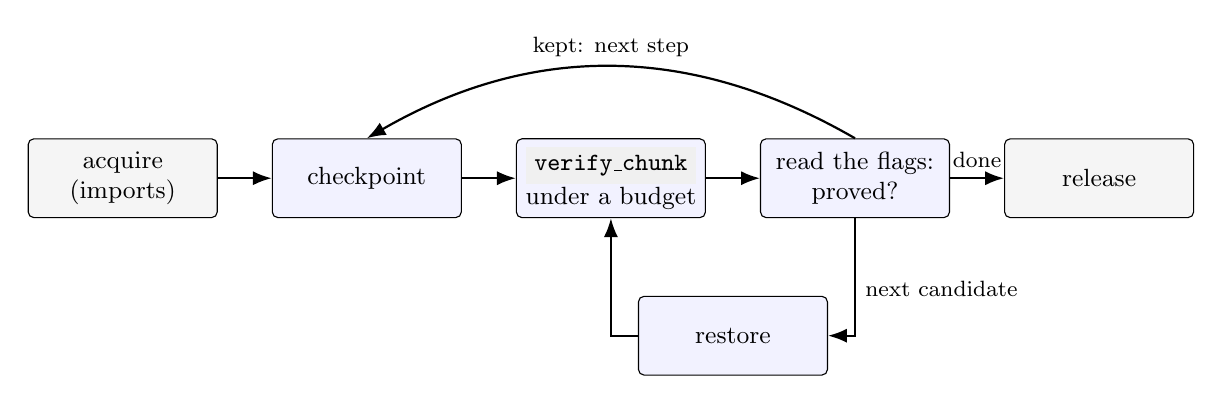
\begin{tikzpicture}[
  x=1cm, y=1cm, font=\small,
  box/.style={draw, rounded corners=2pt, align=center, minimum height=10mm,
    minimum width=24mm, inner sep=3pt, fill=blue!5},
  ends/.style={box, fill=gray!8},
  arr/.style={-{Latex[length=2.4mm]}, thick},
  lbl/.style={font=\footnotesize}
]
\node[ends] (acq) at (0,0)     {acquire\\(imports)};
\node[box]  (cp)  at (3.1,0)   {checkpoint};
\node[box]  (ver) at (6.2,0)   {\code{verify\_chunk}\\under a budget};
\node[box]  (fl)  at (9.3,0)   {read the flags:\\proved?};
\node[ends] (rel) at (12.4,0)  {release};
\node[box]  (res) at (7.75,-2) {restore};
\draw[arr] (acq) -- (cp);
\draw[arr] (cp) -- (ver);
\draw[arr] (ver) -- (fl);
\draw[arr] (fl) -- node[above, lbl] {done} (rel);
\draw[arr] (fl.south) |- node[pos=0.3, right, lbl] {next candidate} (res.east);
\draw[arr] (res.west) -| (ver.south);
\draw[arr] (fl.north) to[out=150, in=30] node[above, lbl] {kept: next step} (cp.north);
\end{tikzpicture}
\caption{A rollout as a sequence of IPS calls. At a proof state the loop
  takes a checkpoint and submits a candidate under a budget. A chunk that
  fails or times out is undone by the server; one that is kept but does
  not prove is undone by a restore before the next candidate; a kept step
  becomes the next state. The loop never starts a session to branch.}
\label{fig:rollout}
\end{figure}

\subsection{Results}
\label{sec:training-measured}

All numbers come from one series of runs on the host of
Section~\ref{sec:serving-measured} (32 cores, 128\,GB, Isabelle2026-RC2).
The workload is the HOL-Analysis library: 93 theories, 11\,984 top-level
blocks, 166\,438 commands. One replay of the library at one worker, the
\emph{census}, proved every block; its times are the reference for every
slowdown below. Each theory runs on a session acquired with its own
imports, as in a curriculum whose problems differ in imports. No model
runs: the candidates are scripted, so the rates are the server's share of
a training loop. Appendix~\ref{app:bench-training} gives the method and
the raw results.

\paragraph{Throughput.} One worker verified 132 chunks (1\,607 commands)
per minute. Thirty-two workers verified 3\,181 chunks per minute, 24 times
as many, while the median call slowed only from 0.41 to 0.52\,s and no
call timed out (Figure~\ref{fig:throughput}). Counting each theory's
session acquisition as well, the rate at 32 workers is 899 chunks per
minute. A cold HOL-Analysis start takes 6\,s on an idle host; it took
8\,s at 8 workers, 34\,s at 16 and 157\,s at 32 (medians), with no
request refused, because the host is then CPU-bound: the provers used
17.7 cores on average and the gateway JVM 4.6, and a start, which is one
ML thread loading a 1.3\,GB heap, waits behind the parallel proof checking
of the other sessions. Acquisition is therefore 10--14\,\% of a worker's
time up to 8 workers, 30\,\% at 16 and 64\,\% at 32. Memory was not the
limit: 29\,GB at the peak. A loop whose problems share imports keeps its
sessions and pays none of this (a warm hit takes 2\,ms); one whose
problems differ in imports should expect the lower curve, or start its
sessions before the clock.

\begin{figure}[!htb]
\centering
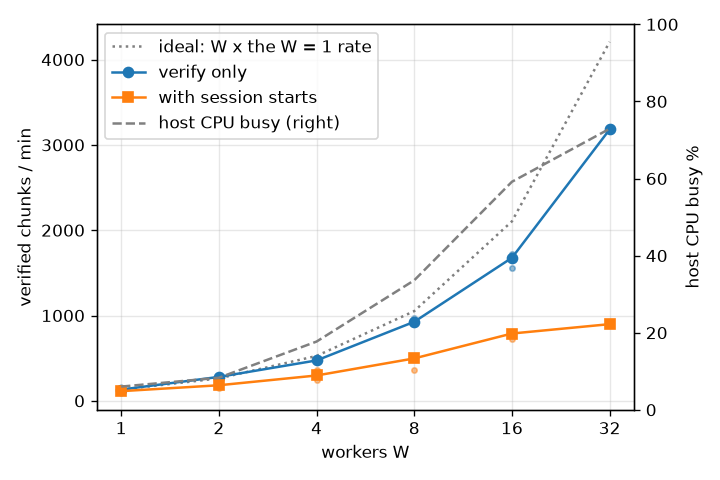
\includegraphics[width=0.8\textwidth]{figures/training_throughput.png}
\caption{Verified chunks per minute against the number of workers, with
  and without each theory's session acquisition, and the host's CPU
  utilisation (dashed, right axis). Three repeats per point, 8 theories
  per worker.}
\label{fig:throughput}
\end{figure}

Table~\ref{tab:rollouts} gives the same measurement for two scripted
rollout loops (Figure~\ref{fig:rollout}): a \emph{whole-proof} loop that
submits eight candidate proofs per theorem, five of which can prove, and
restores the checkpoint after each; and a \emph{step-level} loop that at
every proof command tries two alternatives before the corpus step, with
a checkpoint and restore around each. At one worker the whole-proof loop
runs 6\,436 rollouts per hour and the step-level loop 2\,343 verified
steps per hour; 32 workers run 5.4 and 8.6 times as many. The time a
worker spends on one rollout does not change with the number of workers
(the two ``per rollout'' columns): a worker's loop runs as fast at 32 as
alone, and the rate stops short of 32 times for the reason above, the
session starts. Checkpoint and restore took 3 and 4\,ms in every cell,
and no check of the document's source after a restore failed.

\begin{table}[!htb]
\centering\small
\setlength{\tabcolsep}{4pt}
\begin{tabular}{@{}r rrr rrr r@{}}
\toprule
 & \multicolumn{3}{c}{Whole-proof rollouts} & \multicolumn{3}{c}{Step-level paths} & \\
\cmidrule(lr){2-4} \cmidrule(lr){5-7}
W & per hour & proved/h & s per rollout & per hour & steps/h & s per path & Setup share \\
\midrule
1  & 6\,436  & 954   & 0.60 & 596   & 2\,343  & 3.67 & 0.22 / 0.36 \\
8  & 20\,778 & 2\,839 & 0.60 & 1\,613 & 15\,243 & 3.65 & 0.30 / 0.36 \\
32 & 34\,518 & 4\,798 & 0.61 & 2\,071 & 20\,042 & 3.67 & 0.68 / 0.62 \\
\bottomrule
\end{tabular}
\caption{Scripted rollout loops at W workers, two repeats each. Rates
  are end to end: session acquisition, entering the theory and replaying
  up to each problem included. ``s per rollout'' is a worker's loop time
  per rollout on the theories every cell shares, the like-for-like
  comparison across W. Setup share is the fraction of a worker's time in
  acquisition, entering and replaying to the problems (whole-proof /
  step-level). No rollout ended in a memory, prover-death or session
  error; the candidates' timeout share was 0.5--2\,\%.}
\label{tab:rollouts}
\end{table}

\paragraph{Latency.} Table~\ref{tab:latency} gives the time of one
\code{verify\_chunk} call by chunk size. A single command costs 0.31\,s,
the call's fixed cost: the server re-reads the document every 0.1\,s
until the chunk has settled, then asks the prover whether a proof is
still open. The cost per command falls to 23\,ms in chunks of ten or
more commands, because the prover checks a chunk's proofs in parallel.
Eight workers add nothing to the median and 0.2--0.3\,s to the p95.

\begin{table}[!htb]
\centering\small
\begin{tabular}{@{}l r rr rr r@{}}
\toprule
 & & \multicolumn{2}{c}{W = 1} & \multicolumn{2}{c}{W = 8} & \\
\cmidrule(lr){3-4} \cmidrule(lr){5-6}
Chunk size & calls (W = 1) & p50 & p95 & p50 & p95 & ms per command \\
\midrule
1 command   & 290   & 0.31\,s & 0.63\,s & 0.31\,s & 0.82\,s & 308 \\
2--9 commands & 2\,006 & 0.41\,s & 0.93\,s & 0.41\,s & 1.03\,s & 144 \\
10+ commands & 974   & 0.52\,s & 1.28\,s & 0.62\,s & 1.61\,s & 23 \\
\bottomrule
\end{tabular}
\caption{\code{verify\_chunk} latency by chunk size, from the throughput
  cells at 1 and 8 workers (three repeats each; no call timed out). The
  last column is the p50 per command at W\,=\,1.}
\label{tab:latency}
\end{table}

\paragraph{Branch cost.} We took 200 proof states across 68 theories,
a third each early, in the middle and late in their files, and at each
measured the three ways of going back to the state after trying the next
block: restoring a checkpoint, rolling back the last submission, and the
alternative a REPL offers, replaying the theory up to the state in a new
theory node or a new session (Figure~\ref{fig:branch},
Table~\ref{tab:branch}). A restore returns in 4\,ms. It returns before
the prover has settled, so we charge it the extra time of the verify
that follows it over the same verify settled: the branch cost is 4\,ms at
the median and 20\,ms on average, and at most 63\,ms for the late states.
Replaying to the same state takes 8\,s at the median for the early
states, 43\,s in the middle and 91\,s late in a file, 13.9, 49.6 and
93.2\,s with a fresh session, so a restore is at least 350 times cheaper
than a replay early in a file and 1\,450 times late in it. The verify
after a restore gave the same report as the first verify in all 1\,000
repeats, and the source matched after all 600 restores and 400 rollbacks.

\begin{figure}[!htb]
\centering
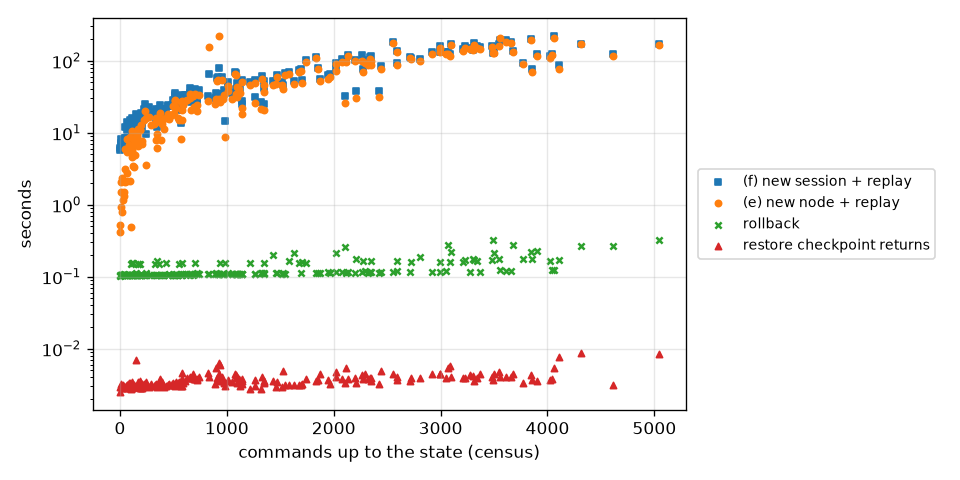
\includegraphics[width=0.9\textwidth]{figures/training_branch_cost.png}
\caption{Going back to a proof state, against the number of commands
  before it: the restore's return time, a rollback, and replaying the
  prefix in a new theory node on the same session or in a new session
  (200 states, log scale).}
\label{fig:branch}
\end{figure}

\begin{table}[!htb]
\centering\small
\begin{tabular}{@{}l rr@{}}
\toprule
Operation & p50 & p95 \\
\midrule
Save a checkpoint & 3\,ms & 4\,ms \\
Restore a checkpoint (returns) & 4\,ms & 5\,ms \\
Branch cost: restore plus its deferred settle & 4\,ms & 200\,ms \\
Roll back the last submission (settled) & 110\,ms & 216\,ms \\
Replay the prefix, new node on the same session & 30\,s & 165\,s \\
Replay the prefix, new session & 35\,s & 169\,s \\
\bottomrule
\end{tabular}
\caption{The cost of going back to a proof state, over 200 states. The
  replay rows pool the three positions; Figure~\ref{fig:branch} shows
  them against the prefix length.}
\label{tab:branch}
\end{table}

\paragraph{Agreement.} The in-session verdict agreed with a cold
\code{isabelle build} on every check we made (Table~\ref{tab:agreement}).
On the 93 theories as written, both accepted all 93. On 200 theorem blocks
sampled across the library, each spliced into its theory in four forms, the
unchanged block was accepted by both in all 200 cases, and the three broken
forms, the proof replaced by \code{sorry}, its last closing step removed,
and a fact name replaced by an undefined one, were rejected by both in all
597 applicable cases. No mutant was proved in-session and rejected cold,
the finding this metric targets, and none was accepted by both. The 693
cold builds took 13.6\,s at the median and 24\,s at p95, four at a time.
On this sample the in-session verdict can be read as a reward without a
cold check; the cold build stays the arbiter where a verdict is final.

\begin{table}[!htb]
\centering\small
\begin{tabular}{@{}l r rrrr@{}}
\toprule
Proof as submitted & n & both accept & in-session only & cold only & both reject \\
\midrule
Theory as written (93 theories) & 93 & 93 & 0 & 0 & 0 \\
Block unchanged & 200 & 200 & 0 & 0 & 0 \\
Proof replaced by \code{sorry} & 200 & 0 & 0 & 0 & 200 \\
Last closing step removed & 200 & 0 & 0 & 0 & 200 \\
A fact name undefined & 197 & 0 & 0 & 0 & 197 \\
\bottomrule
\end{tabular}
\caption{In-session verdict (success, no open proof, no \code{sorry})
  against a cold build of the same text. ``In-session only'' is the unsafe
  disagreement. Three blocks have no fact name to replace.}
\label{tab:agreement}
\end{table}

\paragraph{Bounded step.} We placed 100 looping steps before proved
theorems of 9 theories, 50 of each kind: a rewriting loop
(\code{apply (subst add.commute)+} on an additive goal) and a
\code{metis} call with up to 56 facts on a false goal; each was submitted
under a budget of 5\,s, and the ones that looped again under 30 and
120\,s (Table~\ref{tab:bounded}). Every looping step returned at its
budget with the stuck command named, the server undid it within 0.6\,s at
p95 in every row but one (4.2\,s), the document's source was unchanged
after every attempt, and the next corpus block proved at the census's
speed (0.41\,s median, as in the census). Twelve rewriting seeds failed at
once rather than looping, because the rewrite did not apply to their goal;
they are counted apart. At 8 workers, with 15 looping steps of 120\,s
spread over the workers so that up to seven loops ran at once, the other
workers' blocks ran at the census's speed (median ratio 1.00 over 1\,130
blocks matched against the 8-worker throughput cell) and waited 4--5\,ms
for the server. A long rewriting loop does leave
memory in the prover: 1.2\,GB at the median after a 30\,s loop and 7\,GB
after 120\,s, which the undo does not reclaim; the \code{metis} loops left
130\,MB or less.

\begin{table}[!htb]
\centering\small
\begin{tabular}{@{}l r r r rr r@{}}
\toprule
Looping step & Budget & Attempts & Returned at budget & \multicolumn{2}{c}{Undo p50 / p95} & Memory left, p50 \\
\midrule
\code{metis}, up to 56 facts & 5\,s & 50 & 50 & 0.07\,s & 0.45\,s & 4\,MB \\
 & 30\,s & 10 & 10 & 0.30\,s & 0.60\,s & 127\,MB \\
 & 120\,s & 3 & 3 & 0.28\,s & 0.35\,s & 1\,MB \\
\code{subst} rewrite loop & 5\,s & 38 & 38 & 0.05\,s & 0.52\,s & 4\,MB \\
 & 30\,s & 8 & 8 & 0.54\,s & 4.21\,s & 1\,181\,MB \\
 & 120\,s & 1 & 1 & 0.35\,s & 0.35\,s & 7\,116\,MB \\
\bottomrule
\end{tabular}
\caption{Looping steps under a budget, one worker. Undo is the wall
  time past the budget until the call returned with the step undone.
  Memory left is the prover's resident set after the attempt minus before
  it. Twelve of the 50 rewrite seeds did not loop and are left out.}
\label{tab:bounded}
\end{table}

\subsection{Caveats}

Imports are fixed when a session is acquired, so a curriculum that mixes
import sets needs a session per set or one session on a superset; at 32
workers starting a session per theory, the starts take two thirds of a
worker's time, so a loop should group its problems by imports and keep
the sessions. A looping rewrite leaves memory in the prover that the undo
does not reclaim; a loop that sees repeated timeouts on a session should
release it and acquire a fresh one, which the memory gate will admit on the
reclaimed memory. The one-command mode is sequential; a loop that wants
Isabelle's parallel checking should submit chunks. A budget expiry undoes
the submission silently from the document's point of view: the timeout is
in the response, and a loop that ignores it submits its next step to an
older state than it expects. The in-session verdict agreed with the cold
build on every check here; the cold build remains the arbiter where a
verdict is final, and a reward computed in-session should still be
spot-checked against it on a new corpus.

% ======================================================================
\section{Multi-agent serving}
\label{sec:serving}

This section is for the operator. It states what a shared host needs
from the service, how IPS provides it, and reports the measurements.

\subsection{Requirements}

An operator runs one host for several agents or harnesses, usually
without knowing how many will be active or what they will import. They
need predictability on four counts.

\paragraph{A known number of sessions and a known wait.} Kimina's
motivation was that earlier tools paid an initialisation cost on every
verification~\cite{santos2025kimina}. For Isabelle the cost is larger:
PISA needed a separate 35\,GB copy of Isabelle per concurrent
process~\cite{jiang2021lisa}. Memory, not cores, limits an Isabelle host,
and a warm hit, a cold start and a heap build differ by orders of
magnitude.

\paragraph{No build in the hot path.} Kimina's header-keyed cache halved
its verification time~\cite{santos2025kimina}. An Isabelle project heap
is far more expensive than a Lean import, so a miss costs minutes rather
than seconds.

\paragraph{Defined behaviour when memory runs out.} Kimina added a
per-worker memory cap after out-of-memory
failures~\cite{santos2025kimina}. An Isabelle host has the same failure
mode with larger processes.

\paragraph{Each client's work kept from the others.} AXLE sandboxes every
request~\cite{xin2026axle}, and the Isabelle community has proposed
container and VM setups for agents~\cite{schaeffeler2026safe}. IPS
isolates by lease rather than by process, which is cheaper and weaker;
the isolation measurement below states what it provides.

\subsection{Design}

The pool keeps a configurable number of sessions warm and reuses them
across clients when imports match. Admission is gated on the container's
memory: above the threshold the pool first evicts the least-recently-used
idle session, then refuses a new session with an explanation, so the host
reports ``busy'' instead of suffering an out-of-memory kill. Leases expire
and idle sessions are reaped, so an agent that crashes or fails to release
does not hold a session indefinitely. Project heaps are built once,
verified by fingerprint, and reused by every later session on that
project. Concurrent Sledgehammer runs are capped by a server-wide limit,
since each run fans out to several external provers. The service exposes
liveness and readiness probes, Prometheus metrics and an administrative
view. All sessions share one server process; a crash of that process is
detected and the pool rebuilt.

Agents reach the pool through either MCP server over stdio or streamable
HTTP, harnesses through the Python client. All use the same HTTP API and
are subject to the same leases and budgets. There is no authentication:
IPS assumes a trusted network (Appendix~\ref{app:deploy}).

\subsection{Results}
\label{sec:serving-measured}

All numbers in this section come from one run on a 32-core, 128\,GB
Ubuntu host with Isabelle2026-RC2, both tools native and nothing else
running; Appendix~\ref{app:bench} gives the method, the workloads and the
per-cell raw results. We took each measurement for IPS and, under
identical conditions, for PIDE MCP. This section reports the IPS numbers;
Section~\ref{sec:comparison} reads the two side by side.

\paragraph{Memory measures.} We report memory two ways. The first is the
\emph{proportional set size} (PSS) of the tool's processes, summed over
them: PSS counts a physical page shared by $n$ processes as $1/n$ for
each, so the sum is the memory those processes occupy without counting a
shared page twice, which a sum of the resident set size (RSS) would do and
the unique set size (USS) would avoid only by leaving shared pages out.
For the provers the three agree within 2\,\%: Poly/ML loads the heap image
into its own memory rather than sharing it with the other provers, so a
prover shares only about 13\,MB and its cost is almost entirely private.
The second is
\emph{host used}, \code{MemTotal} minus \code{MemAvailable}, which is the
kernel's own account of what the machine has lost, page cache included,
reported as the change over the cell's baseline. PSS attributes memory to
processes; host used checks that nothing escaped the attribution. Under a
memory limit we also read the cgroup's own counters (\code{memory.current},
\code{memory.peak}, \code{oom\_kill}), since those are what the limit is
enforced on. Appendix~\ref{app:bench} has the definitions in full.

\paragraph{Capacity.} Figure~\ref{fig:capacity} plots host memory against
the number of concurrent sessions for three heaps, each session holding a
checked theory, three repeats per point. The curves are straight to
k\,=\,32. A least-squares fit (Table~\ref{tab:capacity}) separates the
pool's fixed cost, one server process and one gateway JVM, from the cost
of one more session: 894\,MB on HOL, 1084\,MB on HOL-Library and
1271\,MB on HOL-Analysis, which is the prover alone. The gateway JVM
grows from 3.6\,GB at one session to 5.3\,GB at 32, so the fixed cost is
not constant, but its growth is small against the sessions. A 100\,GB
budget holds 110 HOL, 90 HOL-Library or 77 HOL-Analysis sessions. The
same fit on the processes' summed PSS gives per-session costs within 1\,\%
of the host-used ones, so the process view accounts for everything the
host loses. The concurrent re-check of all k theories
(Figure~\ref{fig:peak}, Appendix~\ref{app:bench}) adds 1--3\,\% to the
settled per-session cost under IPS, because it runs inside each prover's
existing heap; under PIDE MCP it adds 4--28\,\%, most on HOL-Library.

\begin{figure}[!htb]
\centering
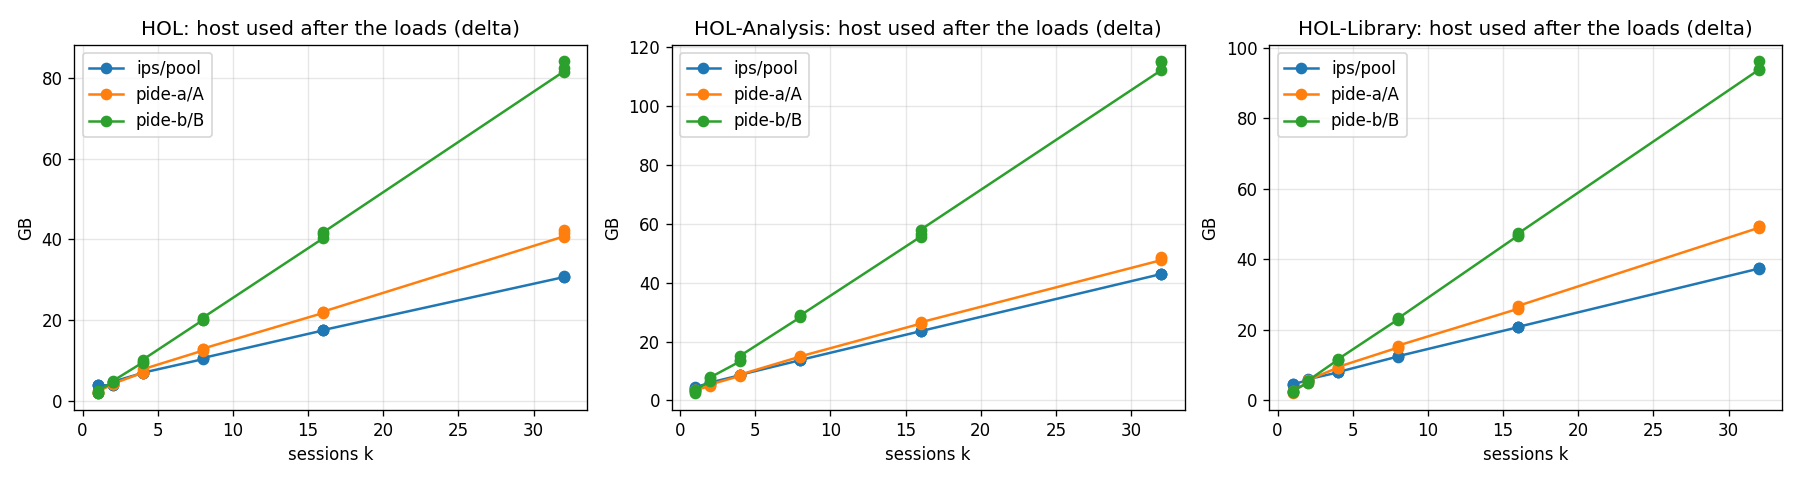
\includegraphics[width=\textwidth]{figures/host_delta_settled_mb.png}
\caption{Host memory used by the tool's processes, above the host's
  baseline, after every session has loaded and checked its theory, against
  the number of sessions k; one panel per heap, three repeats per point.
  IPS: one pool. PIDE MCP A: one process holding k sessions. PIDE MCP B:
  k processes, one session each.}
\label{fig:capacity}
\end{figure}

\begin{table}[!htb]
\centering\small
\setlength{\tabcolsep}{4pt}
\begin{tabular}{@{}llrrrrrrr@{}}
\toprule
Tool & Heap & \shortstack{MB per\\session\\(host)} & \shortstack{Fixed\\MB\\(host)} & \shortstack{MB per\\session\\(PSS)} & \shortstack{Peak MB\\per session\\(PSS)} & \shortstack{Sessions\\per\\100\,GB} & \shortstack{Start\\p50/p95 s} & \shortstack{Load\\p50/p95 s} \\
\midrule
IPS & HOL & 894 & 3183 & 886 & 887 & 110 & 2.3 / 3.9 & 3.1 / 4.1 \\
IPS & HOL-Library & 1084 & 3740 & 1077 & 1092 & 90 & 3.4 / 5.1 & 9.2 / 10.0 \\
IPS & HOL-Analysis & 1271 & 3541 & 1263 & 1267 & 77 & 6.0 / 8.2 & 6.8 / 7.5 \\
\midrule
PIDE MCP A & HOL & 1279 & 1876 & 1266 & 1320 & 78 & 2.0 / 3.2 & 1.2 / 2.2 \\
PIDE MCP A & HOL-Library & 1513 & 2467 & 1495 & 1915 & 66 & 3.0 / 4.3 & 7.2 / 7.4 \\
PIDE MCP A & HOL-Analysis & 1476 & 2671 & 1461 & 1602 & 67 & 5.8 / 7.1 & 1.1 / 1.4 \\
\midrule
PIDE MCP B & HOL & 2665 & $-581$ & 2630 & 2712 & 38 & 3.1 / 3.2 & 1.4 / 1.5 \\
PIDE MCP B & HOL-Library & 3047 & $-620$ & 3017 & 3466 & 33 & 4.1 / 4.2 & 7.3 / 8.3 \\
PIDE MCP B & HOL-Analysis & 3660 & $-232$ & 3604 & 3753 & 28 & 6.7 / 7.3 & 1.3 / 1.4 \\
\bottomrule
\end{tabular}
\caption{Capacity and latency from the E1 matrix: least-squares marginal
  and fixed memory over k\,=\,1\ldots32 (18 cells per row) on host used
  and on summed PSS after the loads, the marginal PSS at the concurrent
  re-check (peak), sessions in a 100\,GB budget on the host slope, and
  start and load latencies. A negative fixed cost is the intercept of a
  straight fit through points that all carry at least one JVM; PIDE MCP B
  has no process at k\,=\,0. The PSS fixed costs are 3.7--4.3\,GB for IPS,
  2.5--3.3\,GB for PIDE MCP A and 0--0.5\,GB for PIDE MCP B
  (Appendix~\ref{app:bench}).}
\label{tab:capacity}
\end{table}

\paragraph{Acquire latency.} Table~\ref{tab:acquire} separates the three
cases. A warm hit, a released session handed to the next client with the
same imports, takes 2\,ms and returned the same session in all 36 trials.
A cold start on a built heap takes 2 to 6 seconds depending on the heap.
A heap build takes minutes: 114\,s for HOL-Library and 360\,s for
HOL-Analysis from the distribution sources on this host, and a project
heap is of the same order. The three cases differ by three orders of
magnitude, which is why the pool and the heap cache exist.

\begin{table}[!htb]
\centering\small
\begin{tabular}{@{}lrrr@{}}
\toprule
 & HOL & HOL-Library & HOL-Analysis \\
\midrule
Warm hit (release, acquire again), p50 & 0.002\,s & 0.002\,s & 0.002\,s \\
Cold start on a built heap, p50 / p95 & 2.3 / 3.9\,s & 3.4 / 5.1\,s & 6.0 / 8.2\,s \\
Heap build from sources (once) & 4\,s\footnotemark & 114\,s & 360\,s \\
\bottomrule
\end{tabular}
\caption{Acquire latency under IPS, by case. Warm hits: 4 sessions, 3
  rounds, every acquire reused the session it had released. Cold starts:
  P1 of the E1 cells. Heap builds: the base heaps on this host.}
\label{tab:acquire}
\end{table}
\footnotetext{HOL was already built by the Isabelle installation; the
figure is the check, not a build.}

\paragraph{Cache hit rate.} Not measured. It needs a mix of projects with
their own heaps and a replayed agent workload, which this round did not
include. Table~\ref{tab:acquire} does fix the size of a miss: a cold
start costs 2 to 6 seconds and a heap build minutes, so one build avoided
per project pays for hundreds of cold starts.

\paragraph{Pressure.} We started the server in a systemd scope with
\code{MemoryMax=48G} and added HOL-Analysis sessions one at a time, each
loading and checking the theory, until the pool refused. IPS admitted 27
sessions and refused the 28th with HTTP 503 and a body that states the
reason: 38.4\,GB in use (78\,\% of the limit), 10.8\,GB available, and
the next session's 4\,GB estimate would cross the 85\,\% threshold; every
running session was leased, so none was evictable; retry in 5\,s. No
process died (\code{oom\_kill} stayed 0; the scope's peak was 38.4\,GB).
After the client released half of its sessions, the next session was
admitted and loaded 8.4\,s later.

\paragraph{Isolation.} With 8 HOL sessions leased, we killed the newest
session's prover process with SIGKILL and asked every session to re-check
its theory within 30\,s. The other 7 answered. The victim's session
returned ``prover process died, the session has been discarded'', and
its slot went back to the pool. The gateway and the server process were
unaffected. A prover death is thus one client's failure, reported as
such. Cross-lease requests, the other half of isolation, are refused by
the lease check; we did not measure them here.

\subsection{Caveats}

The trusted-network assumption is real: anyone who can reach the port can
acquire sessions and, if the ML-command guard is switched off, run
arbitrary code inside Isabelle. Run IPS behind a network boundary or an
authenticating reverse proxy. The administrative page inlines its token
in the rendered page, a known deferred issue
(Section~\ref{sec:limitations}). All sessions share one server process,
so recovery after a crash means every client loses its session at once
and must re-acquire. The admission gate refuses on an \emph{estimate} of
the next session's size; with 10\,GB still free it refused rather than
risk a kill, and an operator who wants that margin used can lower the
estimate. A project heap is rebuilt only on request, so an operator who
updates a project's sources should trigger the rebuild rather than wait
for a client to receive a stale-heap error.

% ======================================================================
\section{Comparison with PIDE MCP}
\label{sec:comparison}

IPS and PIDE MCP~\cite{kappelmann2026pidemcp} are the two headless PIDE
connectors for Isabelle. Both start an Isabelle session without an
editor, drive it through the document model, and expose it to a language
model over MCP; neither is a REPL. They were built for different readers.
This section names the design choices on which they differ and why each
is right for its reader, reports the measurements we took for both under
the same conditions, and lists what each can do that the other cannot.
Appendix~\ref{app:inventory} gives the full inventory.

\subsection{Design choices}

\paragraph{Document ownership.} IPS owns each session's document as a
string the server appends to; the client never sees a file. That makes a
chunk a transaction (undone as a unit on failure), a checkpoint a snapshot
and a restore exact; it also fixes the imports at session start and limits
a session to one theory. PIDE MCP treats the files of a project on disk as
the document: the agent edits them, the server resolves dependencies and
reports positioned messages. That gives project scope, file editing and
co-presence with a human's editor; it rules out transactions, since a file
is not undone.

\paragraph{Time.} PIDE MCP ``decidedly does not block on checking and
does not use timeouts for its core tools'': an edit returns when PIDE has
accepted it, the agent polls a snapshot, and a running check can be
cancelled through the protocol. IPS bounds every wait, and a submission
that exceeds its budget is undone and reported as a timeout. The first
choice suits an agent that can wait, poll and cancel; the second suits a
loop with a fixed worker pool that cannot afford to lose one.

\paragraph{Resource decisions.} IPS has a pool with leases, idle and
lease timeouts, LRU eviction, a memory admission gate and a Sledgehammer
cap. PIDE MCP has none of these; it reports session statistics and leaves
the decisions to whoever runs it. For one agent on one machine that is
the right amount of machinery. For many agents on one host, it is the
difference the next subsection measures.

\subsection{Measurements}

We ran every experiment of Section~\ref{sec:serving-measured} for PIDE
MCP on the same host, Isabelle build, heap cap and workloads, in two
shapes. \emph{Topology A} is PIDE MCP as designed: one process holding k
sessions. \emph{Topology B} gives every agent its own PIDE MCP process,
which is how a group of independent agents would use it without further
infrastructure; it is a cost study of that arrangement, not a defect of
the tool.

\paragraph{Memory per session.} Under topology A a session costs
1279\,MB on HOL, 1513\,MB on HOL-Library and 1476\,MB on HOL-Analysis,
against 894, 1084 and 1271\,MB under IPS (Table~\ref{tab:capacity}):
0.2 to 0.4\,GB more per session, and 67--78 rather than 77--110 sessions
in 100\,GB. The gap is inside the prover processes, not the JVMs: at
every k a PIDE MCP~A prover holds 1.09--1.15\,GB on HOL and 1.38--1.39\,GB
on HOL-Analysis, an IPS prover 0.80 and 1.19\,GB, while the two tools' JVMs
are within 0.4\,GB of each other in total. The cause is the PIDE
perspective. PIDE MCP's \code{edit} marks the edited range and 50 lines
around it as visible (option \code{pide\_mcp\_range\_context}), and our
workload writes the whole theory in one edit, so PIDE runs its print
functions, such as the proof state after each command, for every command
and keeps their output in the prover's document state. IPS declares its
nodes required with an empty visible range and computes proof states on
demand through overlays. The extra memory is the price of output PIDE
MCP's agents read, not overhead; we infer the cause from the code and did
not isolate it in a run. The two tools' session options do not explain
it: IPS's \code{parallel\_proofs=2} can only add memory, and its
\code{threads} setting has no effect. PIDE MCP's fixed cost is lower (1.9--2.7\,GB against
3.2--3.7\,GB): its JVM starts at 1.5\,GB and grows to 5.1\,GB at 32
sessions, where the IPS gateway starts at 3.6\,GB and ends at 5.3\,GB.
For a handful of sessions PIDE MCP A is the smaller deployment; above
about eight sessions IPS is. Under topology B a session costs
2.7--3.7\,GB, three times IPS, because every agent pays a 1.5--2.3\,GB
JVM; 32 HOL-Analysis agents used 118--122\,GB of the 128\,GB host.

\paragraph{Latency.} Cold starts are equal within noise (2--7\,s,
Table~\ref{tab:capacity}). Loading and checking the theory reports lower
for PIDE MCP (1.1--1.4\,s on HOL and HOL-Analysis against 3.1 and 6.8\,s
for IPS; 7.2 against 9.2\,s on HOL-Library). The two timings do not
measure the same thing. IPS's load waits for every command to settle and
assembles a per-command report before returning; PIDE MCP's edit returns
on acceptance, and the experiment then polled \code{get\_state} once a
second until the counts stopped moving, so the PIDE MCP figure is a lower
bound on the time to a usable verdict. The concurrent re-check of all k
theories at k\,=\,32 took a p95 of 3--17\,s under IPS and 10--24\,s
under PIDE MCP A.

\paragraph{Throughput.} On the training workload of
Section~\ref{sec:training-measured}, with the same theories, census and
heap, and each theory on a fresh session started inside the timed window
for both tools, PIDE MCP's edit-and-settle loop (append a block, poll
\code{get\_state} every 0.1\,s until it settles) and IPS's
\code{verify\_chunk} were level at one worker: 135 against 132 chunks per
minute, 116 against 113 with the session starts counted. At eight workers
IPS verified 926 chunks per minute against 813, and 497 against 381 with
the starts. The two calls do not do the same work. \code{verify\_chunk}
undoes a chunk that fails and, after one that succeeds, asks the prover
whether a proof is still open, about one 0.1\,s poll per call, and
returns a verdict; the PIDE MCP loop returns command counts that the
client reads as one. PIDE MCP cannot cancel a block that does not settle,
so such a block ends its theory (one per cell here), and because it names
each theory after its scratch file, the 1\,\% of blocks that refer to
their own theory fail under it.

\paragraph{Under a memory limit.} With \code{MemoryMax=48G} on
HOL-Analysis, IPS admitted 27 sessions and refused the 28th with a reason,
losing nothing. PIDE MCP B admitted 13: the scope reached its limit, and
the kernel killed four of the thirteen MCP processes to make room, so
four agents lost their sessions without any message from the tool, and
the thirteenth was admitted on their memory (Table~\ref{tab:pressure}).
Both tools recovered a new session about 8\,s after half the sessions
were released. We did not run topology A under the limit: with one
process, the first kernel kill ends every session at once, which is the
same outcome in fewer steps.

\paragraph{Isolation.} With one prover among 8 killed, the other 7
sessions answered under all three arrangements. IPS names the cause
(``prover process died'') and frees the slot; PIDE MCP reports the session
as no longer running. Under topology B all eight MCP processes survived
their provers. On this test the tools are equal.

\begin{table}[!htb]
\centering\small
\begin{tabularx}{\textwidth}{@{}>{\raggedright\arraybackslash}p{4.3cm} >{\raggedright\arraybackslash}X >{\raggedright\arraybackslash}X@{}}
\toprule
 & IPS (pool) & PIDE MCP B (one process per session) \\
\midrule
Sessions admitted before the stop & 27 & 13 \\
How it stopped & 28th refused: HTTP 503, \code{memory\_pressure} & kernel OOM kill inside the scope \\
Scope memory at the stop & 38.4\,GB (78\,\%); peak 38.4\,GB & 48.0\,GB (the limit); peak 48.0\,GB \\
Processes lost & none & 4 MCP JVMs and 3 provers: 4 of 13 sessions \\
Recovery after releasing half & 8.4\,s & 8.6\,s \\
\bottomrule
\end{tabularx}
\caption{E3: HOL-Analysis sessions added under a 48\,GB systemd scope
  until the tool refused or a process died.}
\label{tab:pressure}
\end{table}

\subsection{Capabilities}

\paragraph{Only PIDE MCP.} A project of many theories with dependency
resolution; the agent editing files, with messages at line and column; a
visible perspective, so only what the agent looks at is printed;
cancellation of a running check and progress notifications; entity search
over a range; a plugin mechanism through Isabelle services; and three
shipped agent skills. Each follows from treating the files as the
document and from not bounding time.

\paragraph{Only IPS.} A pool with leases, reuse, eviction and a memory
admission gate; transactional chunks, checkpoints and rollback; a
verification call with explicit semantics (success, open proof,
\code{sorry}) and a cold build as arbiter; a wall-clock budget on every
call; batch fan-out across the pool; an HTTP API beside MCP; input
hardening (an ML and file-IO denylist, path roots); Prometheus metrics
and probes; and a test suite. Each follows from owning the document and
from serving many clients.

\paragraph{Both.} Headless PIDE sessions with chosen logic and imports;
per-command status; non-invasive state queries; Sledgehammer; a
Sledgehammer-on-every-\code{sorry} pass (IPS's \code{fill\_sorries} job,
PIDE MCP's extension); MCP over stdio.

\subsection{Summary}

On the questions we measured, memory per session, throughput, conduct
under a limit and isolation, IPS does what it was built for, and PIDE
MCP in its intended shape is within 0.2--0.4\,GB per session of it and
level with it on throughput at one worker, 14\,\% behind at eight. The three-fold
gap appears only when each agent runs its own PIDE MCP process, the
arrangement a group of independent agents falls into without a pool; that
gap is the price of a JVM per agent, and it is the number an operator
choosing between one PIDE MCP per agent and one pool needs. On the
questions we did not measure, the interactive agent's desiderata, PIDE MCP
is the more capable tool, and nothing in our measurements says otherwise.
A group running both would use PIDE MCP for interactive work and IPS in
the training cluster; the two share enough (headless PIDE, overlays,
Sledgehammer) that work on one carries to the other.

% ======================================================================
\section{Related connectors}
\label{sec:position}

Connectors between agents and Isabelle fall into five families, each
built for a reader. Kappelmann's taxonomy and
desiderata~\cite{kappelmann2026pidemcp} supply the family names and the
interactive agent's questions; the training reader's and operator's
questions are those of Table~\ref{tab:metrics}.

\begin{itemize}
  \item \textbf{REPL.} PISA and its descendants~\cite{jiang2021lisa},
    qIsabelle, and the Lean REPL and Pantograph~\cite{aniva2025pantograph}
    on the Lean side. One prover process per worker, commands submitted
    one at a time, state held in memory. Built for the training reader
    and still the most common harness in the lineage. Sequential by
    construction, so parallel proof checking is lost~\cite{wenzel2012repl},
    and every branch is a replay or a fresh process.
  \item \textbf{Batch build.} The agent edits files and runs
    \code{isabelle build}, as in the Munkres
    autoformalisation~\cite{bryant2026munkres}. Simple, editor-agnostic,
    and the only family whose verdict is the cold one by construction.
    Not incremental: every attempt re-checks the whole development.
  \item \textbf{Editor-attached PIDE.} Isabelle/Q~\cite{awslabs2026autocorrode}
    attaches an agent to a human's jEdit session. Full PIDE access and
    co-presence in shared memory, at the price of one session, one
    editor, one machine. Built for the interactive agent beside a human.
  \item \textbf{Headless PIDE, one process per agent.} PIDE
    MCP~\cite{kappelmann2026pidemcp}, and Isabelle-MCP as a third-party
    variant. Built for the interactive agent without an editor, and the
    only family meeting all five of the preprint's desiderata.
    Section~\ref{sec:comparison} measures its cost when many agents share
    a host.
  \item \textbf{Pooled service.} Kimina~\cite{santos2025kimina} and
    AXLE~\cite{xin2026axle} in Lean; IPS in Isabelle. A pool of prover
    processes behind HTTP, built for the training reader and the
    operator: throughput, admission, isolation and a bounded call. IPS is
    the first of this family for Isabelle, and the first in either prover
    whose sessions are PIDE documents, which gives it checkpoints,
    rollback and chunk-level parallel checking.
\end{itemize}

Table~\ref{tab:families} summarises the fit. A tick means the family
answers that reader's questions as designed; a tilde means it can be
made to, with work the reader must do; a dash means it does not try. No
family serves all three readers: the interactive agent wants the whole
PIDE surface and no timeouts, the training reader a narrow, bounded,
pooled contract, and the two conflict on document ownership and on time.
The REPL critique applies to IPS in part. Its one-command mode is a REPL
and inherits the sequential cost; its chunk call submits a block as one
PIDE edit with parallel proofs on, and its whole-file check is a batch
build.

\begin{table}[!htb]
\centering\small
\begin{tabular}{@{}lccc@{}}
\toprule
Family & Training reader & Operator & Interactive agent \\
\midrule
REPL & \checkmark & $\sim$ & -- \\
Batch build & $\sim$ & -- & $\sim$ \\
Editor-attached PIDE & -- & -- & \checkmark \\
Headless PIDE per agent & $\sim$ & -- & \checkmark \\
Pooled service (IPS) & \checkmark & \checkmark & $\sim$ \\
\bottomrule
\end{tabular}
\caption{Which connector family serves which reader.}
\label{tab:families}
\end{table}

\paragraph{A worked example: agents in the loop.} The Isabelle-Humanize
project\footnote{\url{https://github.com/FullBackward/Isabelle-Humanize}}
runs a builder/reviewer loop (the RLCR flow of
humanize2\footnote{\url{https://github.com/humanfia/humanize2}}) on
competition problems. Two agent seats (opencode on DeepSeek V4 Pro in
both roles) talk to IPS through the file MCP server over streamable HTTP,
and the flow uses the IPS whole-file check as the arbiter: a problem
counts as solved only when \code{isabelle build} passes with no
\code{sorry} or \code{oops} and the target theorem present. Three
problems were solved end to end: Putnam 2023 A1 (2 review rounds, 3.3\,h
wall, about \$3 of model time), Putnam 2023 B5 (5 rounds, 14.3\,h, about
\$15, with one regression and a replan) and IMO 2026 P1 (one round, a
1059-line theory with all five \code{sorry}s discharged, 4.2\,h, about
\$5). A rerun of IMO 2026 P1 on the IPS build with incremental document
sync and the memory work of this report halved the wall time (7\,391
against 14\,949\,s) and the agent-active time (117 against 248\,min),
cut MCP timeouts from 12 to 0 and diagnostics calls from 47 to 18 at a
median of 0.3\,s, and the arbiter build from 44 to 11\,s. The project's
own caveats apply: one run per problem, a prompt rule that changed between
the two IMO runs, costs at a model price that has since changed, and a
fourth ``solve'' (Putnam 2023 B6) excluded because the benchmark's Isabelle
statement is degenerate. This is an example, not an evaluation: a few
problems with one model measure the agent and the prompt as much as the
connector. It shows that a service built for the first two readers also
serves the third, and that the service's latency reaches the agent's wall
clock.

% ======================================================================
\section{Limitations and roadmap}
\label{sec:limitations}

\paragraph{Trusted network only.} There is no authentication. The
administrative page inlines its token, a known and deferred issue.

\paragraph{Imports are fixed at session creation.} Changing imports means
a new session. Project imports must use qualified heap names.

\paragraph{One theory per session.} There is no multi-file project scope,
and diagnostics are located at command granularity, not at the line within
a command.

\paragraph{No file editing by the connector.} The file MCP server observes
a file the agent edits with its own tools; the stepwise server has no file
at all.

\paragraph{No protocol-level cancellation or progress.} A running call is
bounded only by its budget; the agent cannot cancel it early or watch it
progress.

\paragraph{No plugin mechanism.} Adding a tool means editing the
repository.

\paragraph{One gateway JVM.} It holds every session's backend and grows
with the pool (3.6 to 5.3\,GB over 32 sessions); a crash of it loses
every session at once.

\paragraph{Cold starts under load.} A session start is one ML thread's
work. At 32 workers each starting a session per theory on a CPU-bound
host, a start took 157\,s at the median against 6\,s alone, two thirds
of a worker's time; the pool does not reserve CPU for starts. Grouping
problems by imports and keeping the sessions avoids it.

\paragraph{Memory left by a looping step.} A looping rewrite can leave
gigabytes in the prover after its undo. The memory gate sees the growth
but does not recycle the session; the client must release it.

\paragraph{Numbers are tied to a build.} Every figure in
Sections~\ref{sec:serving} and~\ref{sec:comparison} is for the Isabelle
build, host and commits in Appendix~\ref{app:bench}; Isabelle2026 was a
release candidate when they were taken.

\paragraph{Roadmap.} Cancellation and progress can be had by routing
calls through Isabelle's own query-operation classes, which would also
give sendback resolution for Sledgehammer results. Per-command timing and
a visible-range perspective are small additions to the report IPS already
produces. Entity search and shipped agent skills are the two items from
the headless-PIDE family that cost least to adopt. Packaging the backend
as an Isabelle tool would remove the remaining reflective access to
Isabelle internals. None of these change the document model, which is
the decision both readers depend on.

% ======================================================================
\section{Conclusion}
\label{sec:conclusion}

IPS is a pooled verification service for Isabelle, built for two readers
that existing connectors do not serve: a training loop that needs fast,
bounded, trustworthy verdicts with cheap branching, and an operator who
needs many agents to share one host predictably. One decision serves
both: the server owns each session's document as text it appends to,
which makes rollback and checkpoints cheap and lets every call run under
a budget, at the price of project scope and positioned diagnostics. On a
128\,GB host a session costs 0.9--1.3\,GB and a warm hit 2\,ms. Under a
48\,GB limit the pool admits 27 HOL-Analysis sessions and refuses the
next with a reason, where one PIDE MCP process per agent reaches 13 and
loses four to the kernel. For the training reader, restoring a
checkpoint costs 4\,ms where replaying to the same proof state costs 8
to 93\,s, the in-session verdict agreed with a cold build on all 890
checks, every looping step returned at its budget, and 32 workers
verified 3\,181 chunks per minute. Among Isabelle connectors IPS is the first of
the pooled-service family, and it complements the interactive families
rather than competing with them: PIDE MCP gives a single agent full
access to a project at a per-session cost within 0.2--0.4\,GB of IPS's,
and IPS gives many clients isolated verification at scale.
Appendix~\ref{app:bench} is sufficient to repeat the measurements.

% ======================================================================
\bibliographystyle{plainnat}
\bibliography{references}

% ======================================================================
\appendix

\section{Quickstart and API summary}
\label{app:quickstart}

\paragraph{Running the server.} IPS ships as one container image
parameterised by Isabelle version, with a setup script for Docker and one
for a native Linux host (optionally as a systemd unit). On a machine with
Docker:
\begin{verbatim}
git clone https://github.com/FullBackward/Isabelle-Pool-Server.git
cd Isabelle-Pool-Server
./deploy/setup.sh --verify     # writes .env, builds, starts, proves True
curl http://localhost:8000/readyz   # 200 once the gateway JVM is up
\end{verbatim}
The first build downloads Isabelle and compiles the backend (10--30\,min).
\code{./deploy/native\_setup.sh --system --systemd --verify} does the same
without Docker. Pool size, memory thresholds, the prover heap cap and the
per-call budgets are environment variables in \code{.env}
(Appendix~\ref{app:deploy}).

\paragraph{A session from Python.} The client is a separate package
(\code{pip install -e ./client}, \code{httpx} only). Every call on a session
carries the lease the acquire returned.
\begin{verbatim}
from client.async_client import PoolAsyncClient

async with PoolAsyncClient("http://localhost:8000") as client:
    s = await client.acquire_session(theories=["Main"], field="HOL")
    sid, lease = s["session_id"], s["lease_id"]
    try:
        await client.enter_theory(sid, "T", imports=["Main"], lease_id=lease)
        cp = await client.save_checkpoint(sid, lease_id=lease)
        r = await client.verify_chunk(
            sid, 'lemma l: "x + 0 = x" by simp', timeout=10.0, lease_id=lease)
        proved = r["success"] and not r["proof_open"] and not r["used_sorry"]
        if not proved:
            await client.restore_checkpoint(sid, cp["checkpoint_id"], lease_id=lease)
    finally:
        await client.release_session(sid, lease_id=lease)
\end{verbatim}
\code{verify\_chunk} returns the per-command report (\code{commands},
each with \code{status} and messages, plus \code{timed\_out} and
\code{stuck\_line} on a budget expiry); \code{load\_document} replaces the
whole document, \code{rollback} undoes the last submission, and
\code{verify\_bigstep\_text} is the cold build.

\paragraph{The stepwise MCP server (13 tools).} \code{enter\_theory},
\code{verify\_chunk}, \code{proof\_state}, \code{source},
\code{diagnostic}, \code{sledgehammer}, \code{checkpoint}, \code{restore},
\code{rollback}, \code{close\_theory}, \code{verify\_batch},
\code{list\_my\_sessions}, \code{memory\_status}.
\code{verify\_chunk} is the only tool that executes Isar.

\paragraph{The file MCP server.} The agent edits a theory file
with its own tools; the server re-reads it on every call and keeps the
session in step. Tools cover open, close and sync; diagnostics, goal and
proof state at a line; source, hover and definition; local and global
facts; query and Sledgehammer; checkpoint, restore, rollback and history;
multi-attempt and run-code on scratch sessions; the Sledgehammer-on-every-\code{sorry}
job; and heap build and status. The naming follows
lean-lsp-mcp~\cite{dressler2026leanlspmcp}.

\paragraph{The HTTP API.} Served with an OpenAPI document at
\code{/openapi.json}. The routes a client uses in order: acquire or
create a session; submit a command, a chunk or a whole document; read
state, goals or facts; checkpoint, restore, rollback; release. Batch
verification and the whole-file check are stateless routes that take a
theory and return a verdict. \code{/api/v1/memory} reports the memory
facts behind every admission decision.

\section{Feature inventory}
\label{app:inventory}

Table~\ref{tab:inventory} is the full side-by-side inventory of IPS and
PIDE MCP, the two headless PIDE connectors of Table~\ref{tab:families},
at IPS commit \code{6e4dd6f} and PIDE MCP commit \code{dd46315}
(2026-10-21). The rows were derived from the interaction stack
(who owns the document, how checking is triggered and reported, how state
is read, how time is bounded), from each project's stated goals, and from
what an adopter asks before deploying. A concern is a row only if at least
one codebase or the preprint documents a deliberate decision about it.

\begin{table}[p]
\centering\scriptsize
\begin{tabularx}{\textwidth}{@{}>{\raggedright\arraybackslash}p{3.4cm} >{\raggedright\arraybackslash}X >{\raggedright\arraybackslash}X@{}}
\toprule
Concern & IPS & PIDE MCP \\
\midrule
Sessions per process & pool with leases & named sessions, own logic and options \\
Pooling, reuse, eviction & yes & no \\
Memory and CPU governance & admission gate, caps, Sledgehammer semaphore & statistics only \\
Multi-file project scope & no: one draft node, imports fixed & yes: theories, ML blobs, dependency resolution \\
Agent file editing & no, read-only by design & \code{edit}, \code{create\_file} \\
Co-presence with a human editor & via disk, file MCP only & via disk, second PIDE process \\
Visible perspective & no & last read or edited range plus context \\
Per-command status & command-granularity ranges & with message positions, timing, \code{bad} \\
Verification with explicit semantics & \code{verify\_chunk} flags; cold build & inferred from counts \\
Transactional rollback, checkpoints & yes & no \\
Non-invasive queries & guarded transient command, overlays & edit into file, read, remove \\
Sledgehammer & tip and positioned, semaphore; \code{fill\_sorries} job & opt-in extension, early stop \\
Entity search & hover, definition at a position & \code{find\_entities} over a range \\
Multi-attempt, batch fan-out & yes & scratch theories \\
Cancellation of a running call & edit removal on budget expiry & protocol cancellation \\
Progress notifications & no & yes \\
Bounded waits & everywhere & none on core tools, by design \\
Transport & HTTP; MCP stdio and streamable HTTP & MCP stdio \\
Error model & HTTP status codes; MCP tools return JSON & \code{isError} results, \code{structuredContent} \\
Plugin mechanism & no & Isabelle services \\
Shipped agent guidance & tool docstrings, one prompt & three skills \\
Input hardening & ML and IO denylist with policy switch, path roots & none \\
Observability & metrics, probes, console, \code{/api/v1/memory} & logs, session statistics \\
Automated tests & about 650 test functions & none \\
\bottomrule
\end{tabularx}
\caption{Functional coverage of IPS and PIDE MCP.}
\label{tab:inventory}
\end{table}

\section{Experiment method and raw results}
\label{app:bench}

Everything in this appendix is reproducible from the IPS repository
(\code{evaluation/memory\_scaling/} for the operator's runs,
\code{evaluation/training\_metrics/} for the training reader's; each
one \code{config.yaml}, numbered scripts and a deterministic analysis)
and the raw data: the full results trees are at
\url{https://github.com/FullBackward/Isabelle-Pool-Server-results}
(the memory-scaling tree also as release asset
\code{memscale-2026-10-21b} of the main repository). The appendix
keeps the method and the series the body's figures are drawn from; the
per-cell tables are in the repository.
Every cell has a manifest (phases, per-session timings, environment,
workload checksum, the tool's own report) and a samples file with one row
per second.

\paragraph{Environment.} Host \code{wenda-Amd-Wrx80}: x86\_64, 32 logical
CPUs, 125.6\,GiB MemTotal, Ubuntu with kernel 6.11.0-26, cgroup v2,
systemd user scopes. Isabelle2026-RC2 (id \code{f79fcaa14d19}), one
installation for both tools, \code{ML\_OPTIONS} \code{--minheap 500
--enablegcsharing --maxheap 9216} (the same per-process heap cap for every
prover of both tools), \code{ISABELLE\_TOOL\_JAVA\_OPTIONS} \code{-Xms512m
-Xmx4g -Xss16m}. IPS commit \code{6e4dd6f} with memory management on at
its defaults (pressure threshold 85\,\%, warning 70\,\%, session
estimates 2048 / 3072 / 4096\,MB for the three heaps), pool size 40,
no pre-warmed sessions, \code{parallel\_proofs=2}, \code{threads=4}; a
fresh server in its own systemd scope for every cell. PIDE MCP
\code{isabelle pide\_mcp} (server 0.1.0, commit \code{dd46315}), no
\code{-o} options. Both
tools ran as one unprivileged user with nothing else on the host.

\paragraph{Workloads.} One fixed theory per heap, loaded whole into every
session: \code{CTL.thy} (HOL, 288 commands), \code{Termination.thy}
(HOL-Library), \code{Sum\_Topology.thy} (HOL-Analysis, 163 lines,
importing \code{HOL-Analysis.Abstract\_Topology}). The re-check inserts
\texttt{lemma memscale\_p5\_done: "True" by simp} after the first paragraph
under the same theory name, so every later command is re-checked on the
incremental path.

\paragraph{Memory measures.} Linux gives three sizes for the physical
memory of one process, and they differ in how shared pages are counted.
The kernel keeps one physical copy of a file-backed page (an executable, a
library) and lets every process that maps it share that copy until one
writes to it. \emph{RSS} counts every physical page the process has
mapped, shared or not, so a sum of RSS counts a shared page once per
process. \emph{PSS} counts a page shared by $n$ processes as $1/n$ for
each, so summed over all processes of a tool it equals the physical memory
they occupy; the kernel reports it per process in
\code{/proc/<pid>/smaps\_rollup}. \emph{USS} counts only pages no other
process maps, what the system would recover if that one process exited.
Measured, sharing between provers is small: Poly/ML reads the session's
heap image into its own memory instead of mapping it shared, so each
prover shares about 13\,MB (libraries) and keeps 0.8--1.4\,GB private, and
its RSS, PSS and USS agree within 2\,\%. We still report the sum of PSS
over the tool's processes, which is exact whatever is shared, and never a
single process's PSS across k. Host used (\code{MemTotal} $-$ \code{MemAvailable} from
\code{/proc/meminfo}) is the independent check: its per-session slope
agrees with the PSS slope within 1\,\% in every series of
Table~\ref{tab:capacity}. The cgroup counters \code{memory.current},
\code{memory.peak} and \code{memory.events} \code{oom\_kill} of the
systemd scope the tool runs in are what a memory limit is enforced on and
carry the E3 result.

\paragraph{Procedure (E1).} For each tool, heap and k in
$\{1,2,4,8,16,32\}$, three repeats: P0 baseline (60\,s, 10\,s after the
first cell of a series), P1 start k sessions, P2 idle 60\,s, P3 load the
theory in each session, P4 settle 60\,s, P5 re-check all k concurrently,
P6 stop and a 30\,s tail. One external sampler reads
\code{/proc/<pid>/smaps\_rollup} for every process of the tool once per
second (RSS, PSS, USS, by role), \code{/proc/meminfo} for host used, and
the scope's \code{memory.current}, \code{memory.peak} and
\code{memory.events}. Steady state is the median of the last 30\,s of a
phase; host used is reported as the delta over the cell's own P0. Fits are
least squares over the 18 cells of a series. The runner refuses to start
twice on one results tree, and the analysis rejects a cell whose samples
show another runner's phases (one cell of the first round was re-run for
that reason).

\paragraph{E2--E4.} E2: 4 IPS sessions, released and re-acquired with the
same imports for 3 rounds. E3: sessions added one at a time under a
systemd scope with \code{MemoryMax=48G} (IPS: the server in the scope;
PIDE MCP B: the experiment and its processes in the scope, with
\code{OOMPolicy=continue} so a kernel kill does not end the scope), until
a refusal, a failed load or an \code{oom\_kill}; then half the sessions
released and one more added. E4: 8 HOL sessions, the newest session's
prover killed with SIGKILL, every session asked to answer within 30\,s
(IPS: a re-check through \code{load\_document}; PIDE MCP:
\code{get\_state}).

\paragraph{Raw results, E1.} Table~\ref{tab:raw} gives, for every tool,
heap and k, the median over the three repeats of the host delta and the
summed PSS after the loads, the PSS peak at the re-check, the JVM's PSS,
and the p50 start, load and re-check latencies. Table~\ref{tab:capacity}
in the body is the fit over these points.

\begin{table}[p]
\centering\scriptsize
\setlength{\tabcolsep}{4pt}
\begin{tabular}{@{}llrrrrrrrr@{}}
\toprule
Tool & Heap & k & \shortstack{Host delta\\MB} & \shortstack{PSS\\MB} & \shortstack{PSS peak\\MB} & \shortstack{JVM\\MB} & \shortstack{Start\\s} & \shortstack{Load\\s} & \shortstack{Re-check\\s} \\
\midrule
IPS & HOL & 1 & 3934 & 4528 & 4557 & 3631 & 3.8 & 4.0 & 0.8 \\
IPS & HOL & 2 & 3990 & 4580 & 4592 & 2851 & 3.1 & 3.2 & 0.8 \\
IPS & HOL & 4 & 7078 & 7627 & 7756 & 4236 & 2.4 & 3.1 & 0.9 \\
IPS & HOL & 8 & 10807 & 11267 & 11517 & 4566 & 2.2 & 3.0 & 1.0 \\
IPS & HOL & 16 & 17907 & 18358 & 18450 & 4994 & 2.1 & 3.0 & 1.5 \\
IPS & HOL & 32 & 31488 & 31774 & 31848 & 5132 & 2.1 & 2.9 & 3.2 \\
IPS & HOL-Library & 1 & 4562 & 5135 & 5281 & 4020 & 4.8 & 10.0 & 6.6 \\
IPS & HOL-Library & 2 & 5886 & 6469 & 6706 & 4317 & 4.2 & 9.5 & 6.6 \\
IPS & HOL-Library & 4 & 8036 & 8648 & 9065 & 4410 & 3.7 & 9.3 & 6.8 \\
IPS & HOL-Library & 8 & 12700 & 13270 & 13558 & 4856 & 3.2 & 9.2 & 7.0 \\
IPS & HOL-Library & 16 & 21250 & 21684 & 22407 & 4914 & 3.2 & 9.2 & 8.8 \\
IPS & HOL-Library & 32 & 38312 & 38655 & 39194 & 5148 & 3.1 & 9.2 & 15.8 \\
IPS & HOL-Analysis & 1 & 4187 & 4779 & 4786 & 3490 & 7.7 & 7.2 & 0.9 \\
IPS & HOL-Analysis & 2 & 6110 & 6698 & 6699 & 4183 & 7.0 & 7.0 & 1.0 \\
IPS & HOL-Analysis & 4 & 8886 & 9459 & 9479 & 4502 & 6.1 & 6.8 & 1.1 \\
IPS & HOL-Analysis & 8 & 14005 & 14559 & 14686 & 4706 & 6.0 & 6.7 & 1.5 \\
IPS & HOL-Analysis & 16 & 24093 & 24582 & 24721 & 4976 & 5.8 & 6.7 & 2.6 \\
IPS & HOL-Analysis & 32 & 44023 & 44364 & 44495 & 5180 & 5.8 & 6.7 & 5.0 \\
\midrule
PIDE MCP A & HOL & 1 & 2004 & 2635 & 2838 & 1536 & 3.2 & 1.3 & 1.2 \\
PIDE MCP A & HOL & 2 & 4232 & 4879 & 4976 & 2537 & 2.6 & 1.3 & 1.2 \\
PIDE MCP A & HOL & 4 & 7386 & 7846 & 8574 & 3737 & 2.0 & 1.2 & 1.2 \\
PIDE MCP A & HOL & 8 & 13228 & 13412 & 13790 & 4203 & 1.9 & 1.1 & 1.3 \\
PIDE MCP A & HOL & 16 & 22566 & 22924 & 23612 & 4674 & 1.8 & 1.1 & 2.5 \\
PIDE MCP A & HOL & 32 & 42520 & 42800 & 44284 & 4999 & 1.8 & 1.1 & 11.4 \\
PIDE MCP A & HOL-Library & 1 & 2412 & 2979 & 3612 & 1583 & 4.1 & 7.3 & 6.2 \\
PIDE MCP A & HOL-Library & 2 & 5380 & 5932 & 6771 & 2952 & 3.8 & 7.2 & 7.2 \\
PIDE MCP A & HOL-Library & 4 & 9429 & 9989 & 12010 & 4215 & 3.2 & 7.2 & 7.3 \\
PIDE MCP A & HOL-Library & 8 & 15437 & 15890 & 20054 & 4161 & 2.9 & 7.2 & 9.5 \\
PIDE MCP A & HOL-Library & 16 & 26814 & 27192 & 35385 & 4601 & 2.8 & 7.2 & 14.4 \\
PIDE MCP A & HOL-Library & 32 & 50579 & 50347 & 63592 & 4916 & 2.8 & 7.2 & 23.1 \\
PIDE MCP A & HOL-Analysis & 1 & 3515 & 4078 & 4121 & 2667 & 6.9 & 1.2 & 1.1 \\
PIDE MCP A & HOL-Analysis & 2 & 5334 & 5891 & 6163 & 3100 & 6.3 & 1.2 & 1.2 \\
PIDE MCP A & HOL-Analysis & 4 & 8902 & 9475 & 9714 & 3982 & 6.1 & 1.1 & 1.2 \\
PIDE MCP A & HOL-Analysis & 8 & 15261 & 15656 & 16594 & 4479 & 5.5 & 1.1 & 2.3 \\
PIDE MCP A & HOL-Analysis & 16 & 26870 & 27294 & 29416 & 4691 & 5.7 & 1.1 & 3.9 \\
PIDE MCP A & HOL-Analysis & 32 & 49611 & 49750 & 54329 & 4861 & 5.3 & 1.1 & 9.5 \\
\midrule
PIDE MCP B & HOL & 1 & 2000 & 2624 & 2773 & 1532 & 3.1 & 1.4 & 1.2 \\
PIDE MCP B & HOL & 2 & 4854 & 5314 & 5576 & 3011 & 3.1 & 1.3 & 1.2 \\
PIDE MCP B & HOL & 4 & 9780 & 10575 & 10825 & 6016 & 3.1 & 1.4 & 1.2 \\
PIDE MCP B & HOL & 8 & 20496 & 20689 & 21811 & 12032 & 3.1 & 1.4 & 1.3 \\
PIDE MCP B & HOL & 16 & 42305 & 42286 & 43807 & 23962 & 3.1 & 1.4 & 3.9 \\
PIDE MCP B & HOL & 32 & 84550 & 84318 & 86496 & 47746 & 3.1 & 1.4 & 8.6 \\
PIDE MCP B & HOL-Library & 1 & 2458 & 2986 & 3521 & 1577 & 4.1 & 7.3 & 7.2 \\
PIDE MCP B & HOL-Library & 2 & 5563 & 6080 & 7053 & 3093 & 4.1 & 7.3 & 7.2 \\
PIDE MCP B & HOL-Library & 4 & 11745 & 12147 & 14066 & 6185 & 4.1 & 7.3 & 7.7 \\
PIDE MCP B & HOL-Library & 8 & 23499 & 23746 & 27489 & 12357 & 4.1 & 7.3 & 9.8 \\
PIDE MCP B & HOL-Library & 16 & 47929 & 47854 & 55850 & 24590 & 4.1 & 7.3 & 14.7 \\
PIDE MCP B & HOL-Library & 32 & 96227 & 96119 & 110388 & 49126 & 4.1 & 7.3 & 24.7 \\
PIDE MCP B & HOL-Analysis & 1 & 3195 & 3796 & 3970 & 2385 & 6.9 & 1.3 & 1.2 \\
PIDE MCP B & HOL-Analysis & 2 & 7629 & 8111 & 8430 & 5455 & 6.8 & 1.3 & 1.2 \\
PIDE MCP B & HOL-Analysis & 4 & 14074 & 14526 & 14936 & 9007 & 6.7 & 1.3 & 1.2 \\
PIDE MCP B & HOL-Analysis & 8 & 29421 & 29642 & 30072 & 18770 & 6.7 & 1.3 & 2.3 \\
PIDE MCP B & HOL-Analysis & 16 & 57903 & 57627 & 59280 & 35583 & 6.7 & 1.3 & 4.7 \\
PIDE MCP B & HOL-Analysis & 32 & 117851 & 116454 & 120589 & 71663 & 6.6 & 1.3 & 9.0 \\
\bottomrule
\end{tabular}
\caption{E1 raw results: medians over three repeats per (tool, heap, k).
  Host delta and PSS after the loads (P4), PSS peak at the concurrent
  re-check (P5), the JVM's PSS at P4 (for PIDE MCP B the sum of its k
  JVMs), and p50 latencies of session start (P1), theory load (P3) and
  re-check (P5).}
\label{tab:raw}
\end{table}

\begin{figure}[!htb]
\centering
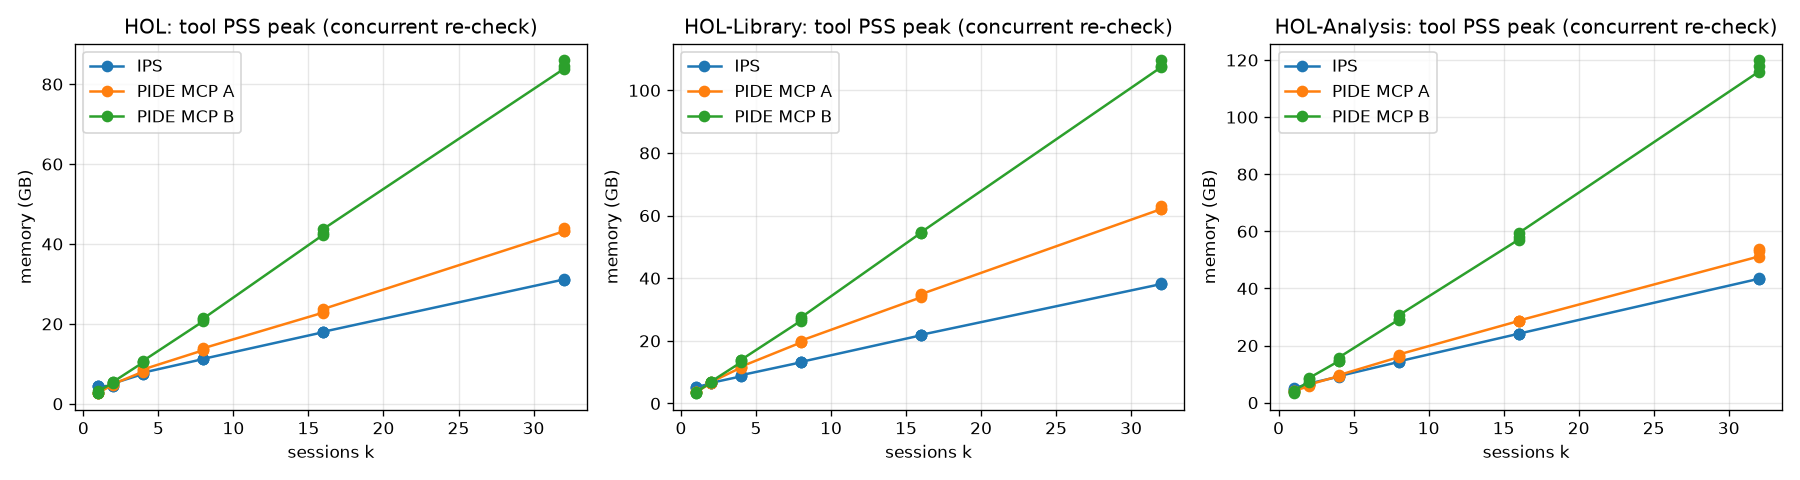
\includegraphics[width=\textwidth]{figures/pss_peak_mb.png}
\caption{Summed PSS of the tool's processes at the concurrent re-check of
  all k theories (P5 peak), against k; one panel per heap, three repeats
  per point.}
\label{fig:peak}
\end{figure}

\paragraph{Raw results, E3.} Table~\ref{tab:raw-e3} gives the scope's
\code{memory.current} after each session loaded. IPS: 27 admitted,
1.2--1.3\,GB per step, the 28th refused at 38.4\,GB with state \texttt{warning}, 38\,382\,MB
used of 49\,152 and 10\,770\,MB available.
PIDE MCP B: 3.4--5.1\,GB per step; at the 12th and 13th sessions the
prover count fell (11, then 9) as the kernel began killing inside the
scope, and the 14th load succeeded with \code{oom\_kill} at 4 and 7
provers left.

\begin{table}[!htb]
\centering\scriptsize
\setlength{\tabcolsep}{3.5pt}
\begin{tabular}{@{}l rrrrrrrrrrrrrr@{}}
\toprule
Session added & 1 & 2 & 3 & 4 & 5 & 6 & 7 & 8 & 9 & 10 & 11 & 12 & 13 & 14 \\
\midrule
IPS, scope MB & 5460 & 6853 & 8120 & 9367 & 10610 & 12074 & 13323 & 14577 & 15831 & 17078 & 18323 & 19606 & 20854 & 22110 \\
PIDE MCP B, scope MB & 6214 & 10257 & 13668 & 17058 & 21249 & 26373 & 31105 & 35752 & 39925 & 44512 & 48731 & 49139 & 49143 & 33935 \\
PIDE MCP B, provers alive & 1 & 2 & 3 & 4 & 5 & 6 & 7 & 8 & 9 & 10 & 11 & 11 & 9 & 7 \\
\bottomrule
\end{tabular}
\caption{E3 under \code{MemoryMax=48G}, HOL-Analysis: the scope's
  \code{memory.current} after each session loaded. IPS continued at the
  same slope to 38\,385\,MB at the 27th session and refused the 28th;
  PIDE MCP B's 14th load succeeded after the kernel had killed four of its
  processes (\code{oom\_kill} 4).}
\label{tab:raw-e3}
\end{table}

\paragraph{Raw results, E2 and E4.} E2: cold start p50 2.2 / 3.1 / 5.8\,s
and warm re-acquire 0.002\,s for HOL / HOL-Library / HOL-Analysis; all
12 re-acquires per heap returned the released session. E4, k\,=\,8 on
HOL: IPS, 7 of 7 others answered, the victim reported ``prover process
died, the session has been discarded''; PIDE MCP A, 7 of 7, the victim
``No running session s7'', the one JVM alive; PIDE MCP B, 7 of 7, the
same message, all 8 JVMs alive.

\paragraph{Training workloads.}
\label{app:bench-training}
The runs of Section~\ref{sec:training-measured} are reproducible from
\code{evaluation/training\_metrics/} in the IPS repository (one
\code{config.yaml}, numbered scripts, a deterministic analysis); the raw
results, every cell's manifest, per-block records, memory and CPU samples
and the server's reports, are the \code{training-metrics/} tree of the
results repository above. Same host and Isabelle build as above; IPS
commit \code{1fe270f}, pool size 40, no pre-warmed sessions,
\code{parallel\_proofs=2}, memory management on with a 1.5\,GB estimate per
HOL-Analysis session, four cold builds at a time. PIDE MCP as above with
\code{parallel\_proofs=2} on its sessions.

\emph{Corpus and census.} The 93 theories of HOL-Analysis in
Isabelle2026-RC2 with their imports qualified, each split into top-level
blocks (11\,984; a block is one top-level command with its proof). The
census replays every theory once at one worker, each on a session with the
theory's imports, with a 600\,s budget per block; it proved all 11\,984
blocks, and its per-block times and command counts key every later
measurement. A block's budget in the experiments is $\min(600,
\max(30, 2n))$\,s for $n$ census commands.

\emph{T1 throughput and T2 latency.} W workers (1 to 32, three repeats),
8 theories each from a seeded assignment that is a prefix across W, each
theory on a fresh session acquired with its imports, replayed block by
block with \code{verify\_chunk}; the clock runs from the first theory to
the last. Table~\ref{tab:t1-series} is the full series. The PIDE MCP row
runs the same assignment at W\,=\,1 and 8 as edit-and-settle.
\emph{T3 branch cost.} 200 proof states, a third each early, in the middle
and late in their theories, each on a session created for it: checkpoint,
verify the next block, three restores each followed by the block, two
rollbacks each followed by the block, then the prefix replayed in a new
theory node and in a new session. \emph{T4 agreement.} Part A: each theory
as written, the census verdict against \code{verify\_bigstep\_text}
(\code{isabelle build} on the heap). Part B: 200 census-proved theorem
blocks, seeded, in four forms (unchanged, \code{sorry}, truncated before
the closing step, first fact name undefined), checked in-session at the
block's position under its budget and rolled back, and cold with the form
spliced into its theory, one mutation per build. \emph{T5 bounded step.}
50 seeds per family placed before census-proved theorems of 9 theories,
tried at 5\,s, the ones that looped again at 30 and 120\,s while the
family's count lasts; a 1.5\,s pause after every attempt for the memory
sampler; at W\,=\,8, two seeds per worker of 120\,s among the worker's
theories. \emph{T6 rollout loops.} W workers (1, 8, 32; two repeats), three
theories each from the T1 assignment; whole-proof: the first 8 proved
theorems of each theory, 8 candidates each (the corpus proof, \code{by
auto} and \code{by simp} twice, \code{sorry}, the proof truncated, a method
that fails at once) under 20\,s, a kept one undone by a restore;
step-level: the first 4 proved theorems of 2 to 40 proof commands, at each
command two alternatives from \{\code{apply auto}, \code{apply simp},
\code{apply -}, \code{by auto}, \code{by simp}\} under 10\,s before the
corpus command. Every cell polls the server's memory tier and samples
memory and CPU per process once a second.

\begin{table}[!htb]
\centering\small
\setlength{\tabcolsep}{4pt}
\begin{tabular}{@{}r rrr rr r rr rr@{}}
\toprule
W & \shortstack{chunks/min\\verify only} & \shortstack{commands\\per min} & \shortstack{chunks/min\\incl.\ acquire} & \shortstack{acquire\\share} & \shortstack{census\\work rate} & \shortstack{slowdown\\vs census} & \shortstack{p50\\s} & \shortstack{p95\\s} & \shortstack{host\\CPU \%} & \shortstack{PSS peak\\GB} \\
\midrule
1  & 132   & 1\,607  & 113 & 0.10 & 0.97 & 1.02 & 0.41 & 0.92 & 6  & 6.5 \\
2  & 281   & 3\,713  & 183 & 0.12 & 1.44 & 1.04 & 0.41 & 0.92 & 8  & 7.5 \\
4  & 474   & 6\,576  & 297 & 0.12 & 2.58 & 1.08 & 0.41 & 1.06 & 18 & 11.3 \\
8  & 927   & 12\,501 & 497 & 0.14 & 4.45 & 1.17 & 0.42 & 1.22 & 34 & 16.0 \\
16 & 1\,677 & 22\,353 & 789 & 0.30 & 7.07 & 1.62 & 0.47 & 1.41 & 59 & 26.5 \\
32 & 3\,181 & 44\,877 & 899 & 0.64 & 8.33 & 3.13 & 0.52 & 1.50 & 73 & 28.3 \\
\bottomrule
\end{tabular}
\caption{T1 at every W (three repeats averaged; no call timed out, no
  theory skipped). Census work rate: the census time of the cell's
  theories over the cell's wall time, the number of single-worker replays
  the cell is worth. Slowdown: the cell's replay time over the census time
  of the same theories, acquisition included.}
\label{tab:t1-series}
\end{table}

\section{Deployment and security}
\label{app:deploy}

\paragraph{Sizing.} About 30\,GB of disk for Isabelle and the heaps. For
memory, budget 3.5\,GB for the server and gateway plus 0.9\,GB per HOL
session, 1.1 per HOL-Library session and 1.3 per HOL-Analysis session at
steady state (Table~\ref{tab:capacity}), and leave the admission gate's
margin on top: it refuses when the next session's estimate would cross
85\,\% of the cgroup limit. The pool size, the number of sessions started
at boot, the idle and lease timeouts, the memory thresholds and session
estimates, the prover heap cap and the per-call budgets are configured
through environment variables documented in the repository's
\code{.env.example}.

\paragraph{Setup.} One Dockerfile parameterised by Isabelle version, with
native-architecture selection and mirror fallback; a setup script for
Docker and one for a native Linux host (optionally as a systemd unit).
Readiness and liveness are exposed as HTTP probes; metrics are exposed for
Prometheus, with a Grafana dashboard in the repository. The memory gate
reads the server's own cgroup, so it sees a Docker memory limit and a
systemd \code{MemoryMax} alike.

\paragraph{Security envelope.} No authentication; the trust boundary is
the network. Every endpoint that accepts Isar text rejects ML, setup and
file-IO commands unless the operator switches the policy off. The
diagnostic endpoint accepts only an allowlist of keywords. Heap project
paths are confined to configured roots, and destructive heap operations
require an administrative token. Measured against the MCP specification's
requirements for input validation, access control and rate
limiting~\cite{mcp2025spec}, IPS meets the first in part and neither of
the others. PIDE MCP states that it includes no safety measures and refers
to a separate set of sandboxed setups~\cite{schaeffeler2026safe}.

\section{How the server works}
\label{app:code}

\paragraph{Tiers.} A Scala backend, packaged as an Isabelle component,
creates headless sessions through Isabelle's server machinery hosted in
its own process; one backend object per session owns a draft theory node
and the edit and rollback bookkeeping. All backends live in one gateway
JVM, reached from Python over a bridge whose calls are serialised per
session, since neither the bridge nor the backend is thread-safe. A
FastAPI server owns the pool and the HTTP API, keeps its event loop free of
prover waits by running backend calls on worker threads, and exposes
metrics and probes. The Python client and the two MCP servers sit above
it.

\paragraph{The owned document.} Each session's document is a string the
backend appends to. Every insert is recorded in a parent-linked chain of
status snapshots, so rollback removes the last insert, a checkpoint is a
snapshot, and restore replays the difference. The theory header is parsed
from the accumulated text and overwritten by a wrapper import so that the
session's imports supply the visible context. Whole-document replacement,
used by the file MCP server, is diffed into sequential edits. Because PIDE
spans for a string node carry no file positions, diagnostics are located
by the owning command's range.

\paragraph{Verification.} The one-command call inserts a command, waits
under a budget for its status, and removes it on expiry. The chunk call
inserts the block as one edit, waits for every command to settle or the
budget to expire, classifies each command, and removes the block if any
command failed or the budget expired. The whole-file check writes the
theory to a temporary session directory, runs \code{isabelle build} with
a content-addressed cache, and returns the result.

\paragraph{State queries.} Goals, in-proof status, local and global
facts, rendered state and Sledgehammer are query operations registered in
Isabelle/ML and invoked from Scala as temporary overlays on the
document's last command~\cite{wenzel2014pide}; the backend polls the
command's results for a finished marker under a budget and then removes
the overlay. Only the diagnostic endpoint inserts a transient command.
PIDE MCP is a headless PIDE front-end in the same sense~\cite{wenzel2019pide};
the two differ in what the document is, not in how PIDE is driven.

\paragraph{Pool, leases, admission.} Sessions are keyed by sorted
imports, base heap and heap fingerprint. A lease is a token presented on
every call; expired and abandoned leases are reaped on a timer, as are idle
sessions. Admission reads the server's own cgroup memory accounting, since
the JVM cannot see the prover processes' memory, estimates the next
session's size by heap, and evicts least-recently-used idle sessions
before refusing; a refusal carries the facts (used, limit, available,
what is leased) so the client can decide what to do. A prover death is
detected on the next call, reported as such, and the session discarded; a
gateway crash restarts the gateway. Project heaps are built with
\code{isabelle build -b} and recorded with a manifest of source
fingerprints; a mismatch returns a stale-heap error.

\paragraph{Where to look.} Session start in
\code{server/repl/src/main/scala/repl/session\_manager.scala}; document
edits in \code{repl\_session.scala} and \code{edit\_utils.scala}; overlay
queries in \code{document\_utils.scala} and \code{src/ml/REPL.ML}; the
per-command report in \code{document\_utils.scala}; the HTTP layer in
\code{server/app}; the pool and memory monitor in
\code{server/app/services}; the guards in \code{server/app/core}; the MCP
servers in \code{mcp\_servers/stepwise} and \code{mcp\_servers/lsp}; the
experiments of Appendix~\ref{app:bench} in
\code{evaluation/memory\_scaling}.

\end{document}
